\documentclass{article}
\usepackage[utf8]{inputenc}
\usepackage{graphicx}
\usepackage{graphicx}

\title{Normalisasi Tabel}
\author{Rizal Ramadhan }
\date{November 2019}

\begin{document}

\maketitle

\section{Normalisasi tabel}
\begin{enumerate}
    \item disini kita akan membuat normalisasi dari table yang akan dibuat.dan sebelum itu kita akan buat saja table nya seperti dibawah ini dan dibuat di excell dan agar lebih mudah gunakan saja sheet pada excell dan di table terdapat Tmahasiswa,Tdosen,Tkuliah,Tnilai,Jadwal
    
        Tmahasiswa
    \ref{excel}
    \begin{center}
         \centering
            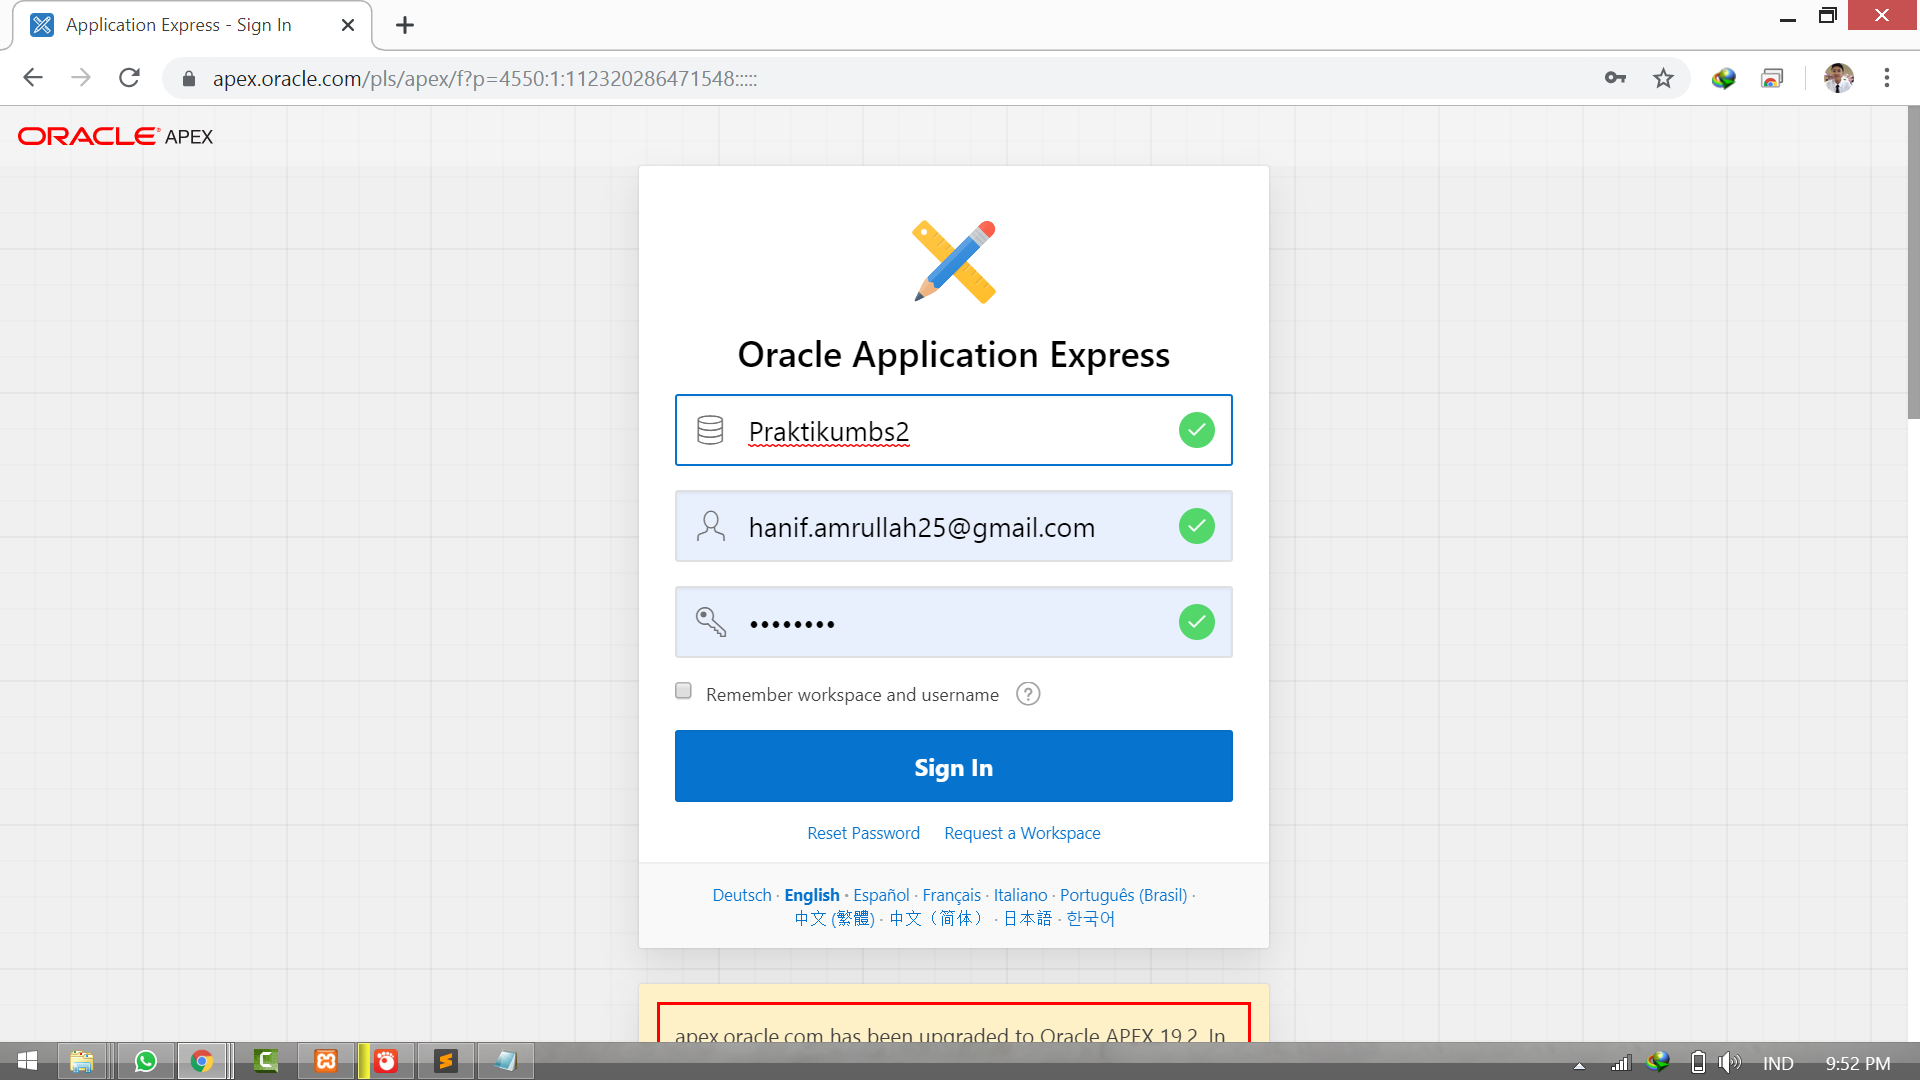
\includegraphics[scale=0.27]{gambar/1.png}
        \caption{Menambahkan Data}
        \label{excel}
    \end{center}
    
        Tdosen
    \ref{excel}
    \begin{center}
         \centering
            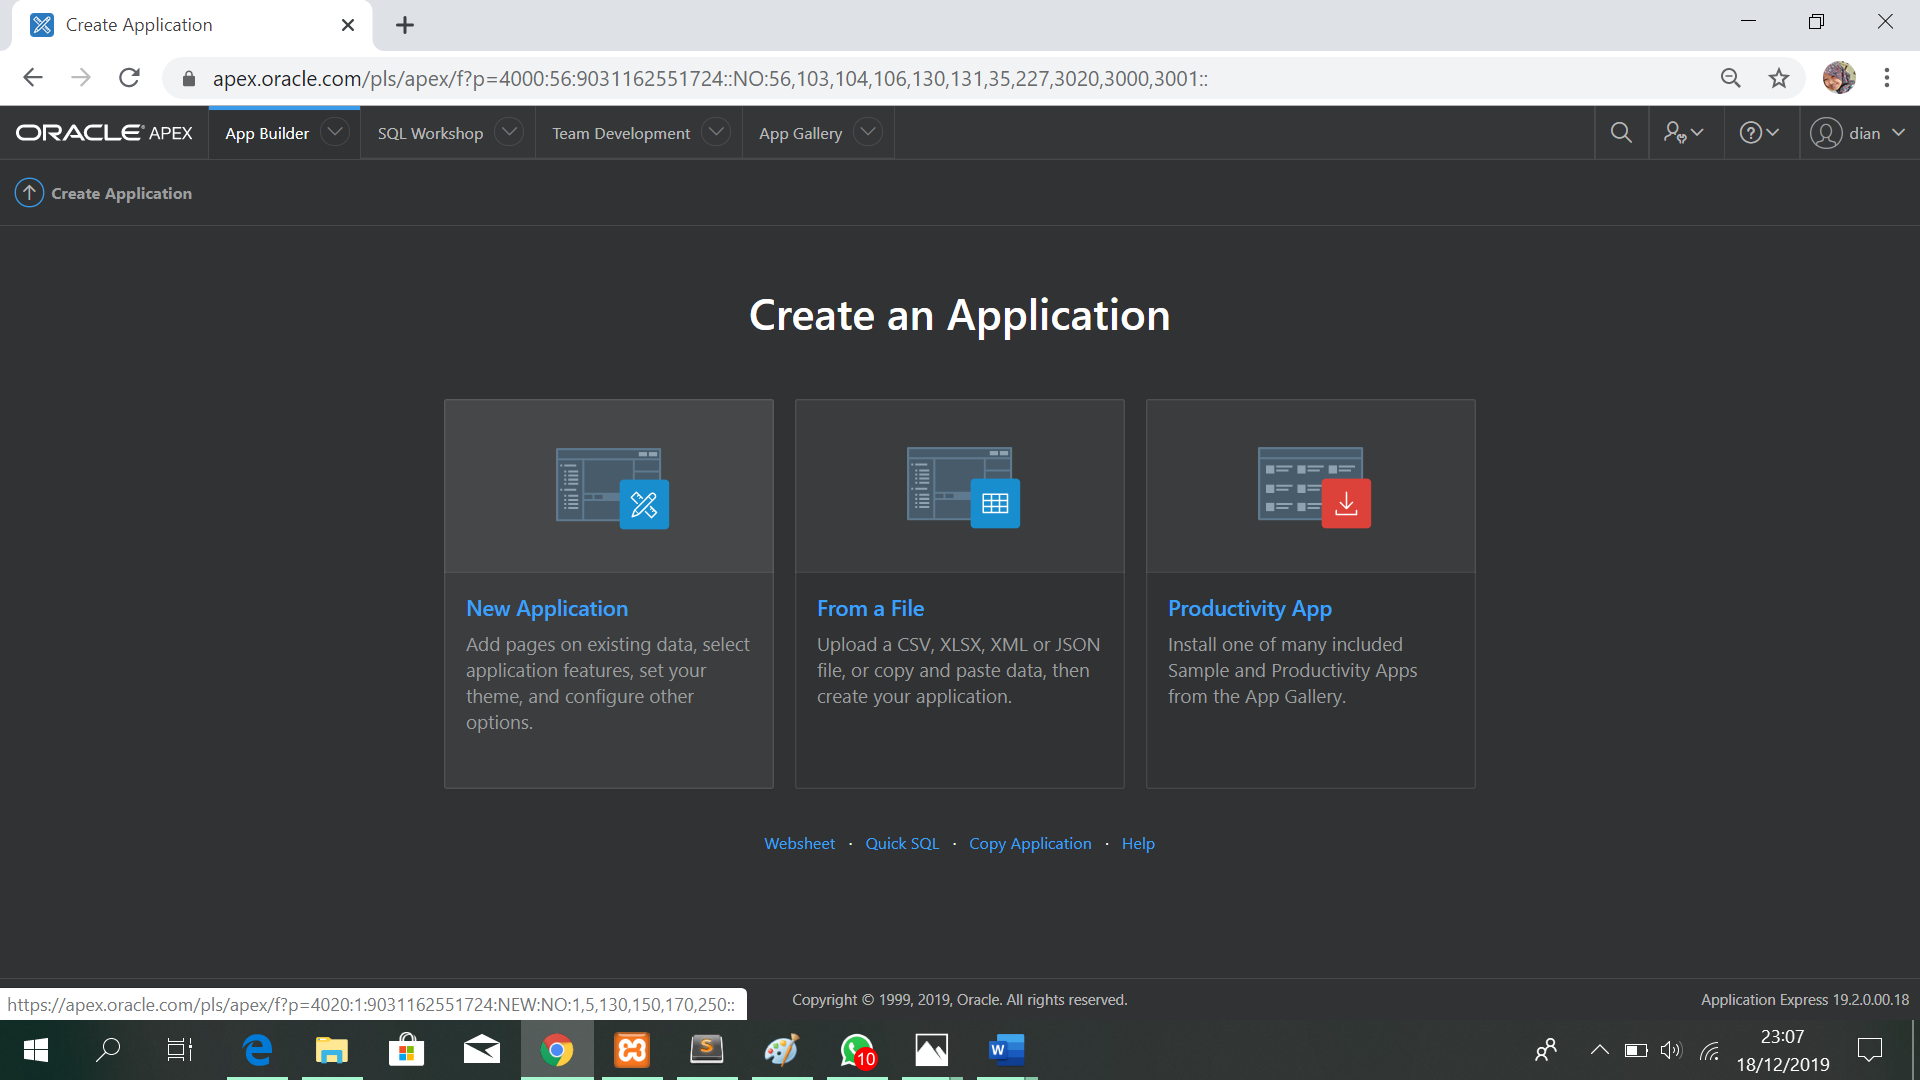
\includegraphics[scale=0.27]{gambar/2.png}
        \caption{Menambahkan Data}
        \label{excel}
    \end{center}
    
        Tkuliah
    \ref{excel}
    \begin{center}
         \centering
            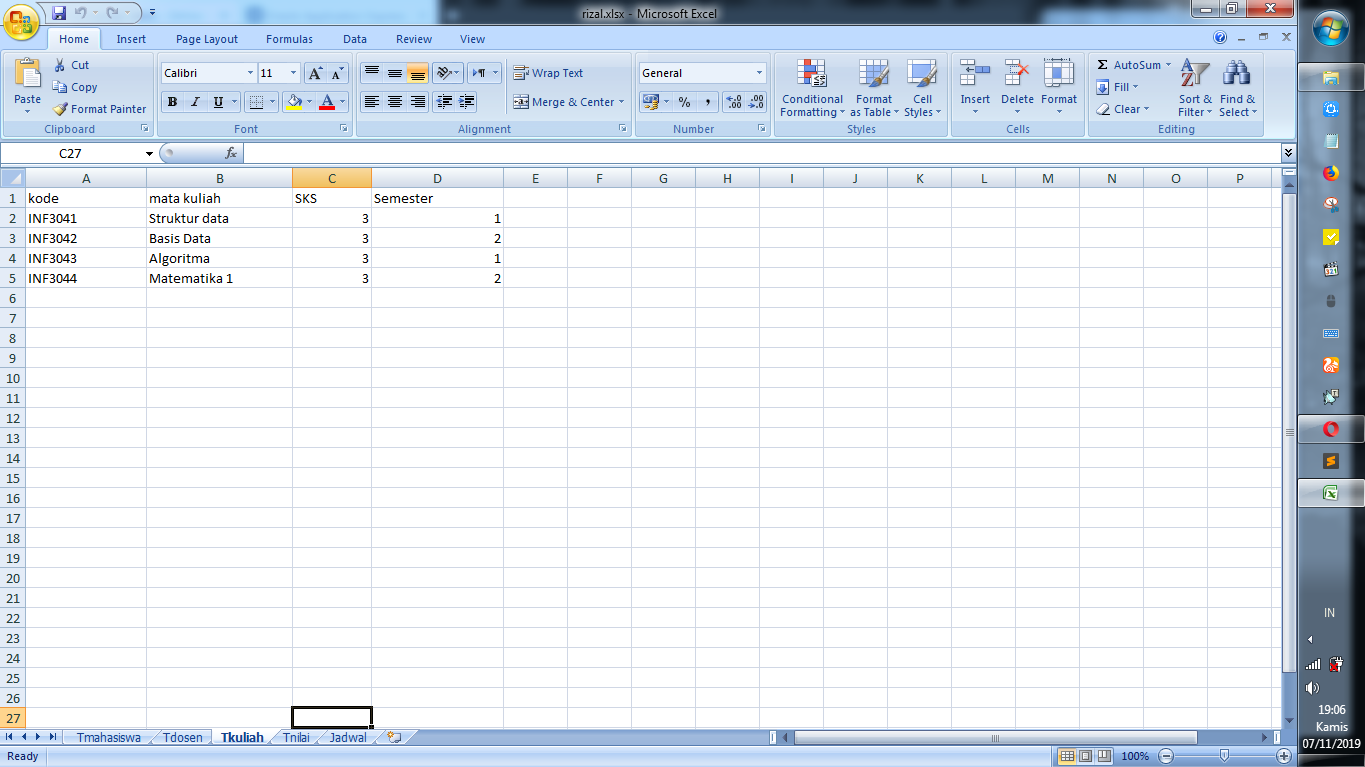
\includegraphics[scale=0.27]{gambar/3.PNG}
        \caption{Menambahkan Data}
        \label{excel}
    \end{center}
    
        Tnilai
    \ref{excel}
    \begin{center}
         \centering
            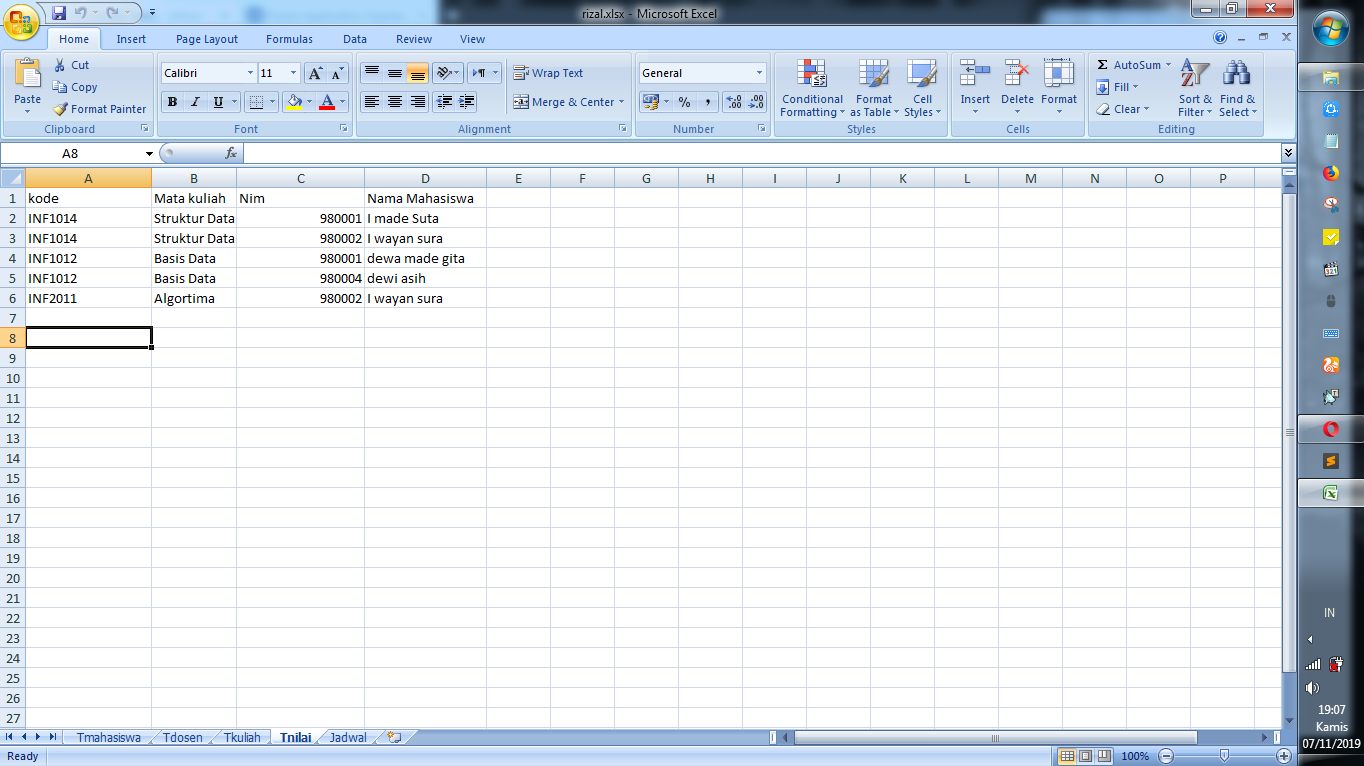
\includegraphics[scale=0.27]{gambar/4.PNG}
        \caption{Menambahkan Data}
        \label{excel}
    \end{center}
    
        Jadwal
    \ref{excel}
    \begin{center}
         \centering
            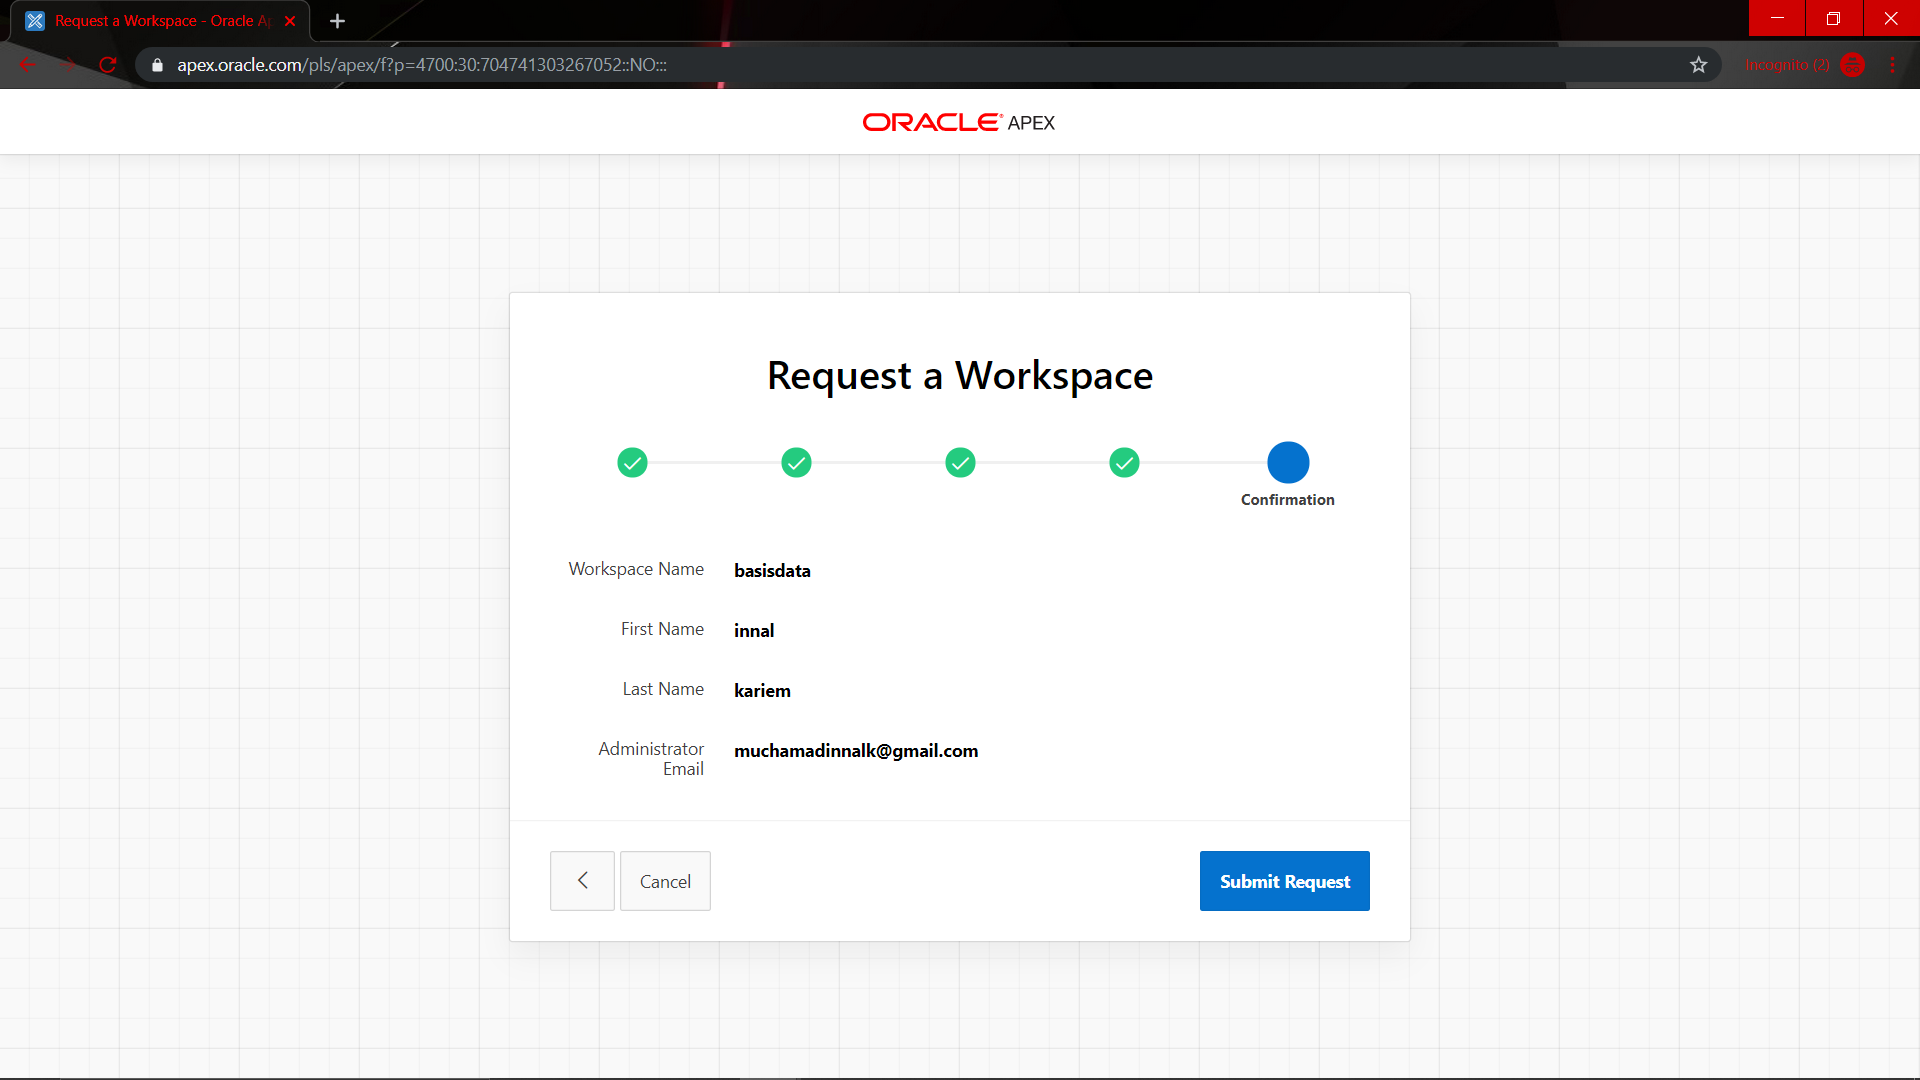
\includegraphics[scale=0.27]{gambar/5.png}
        \caption{Menambahkan Data}
        \label{excel}
    \end{center}
       
     \item langkah selanjutnya adalah cara memasukan table tersebut
     
    masuk kedalam oracle express
      \ref{create}
    \begin{center}
         \centering
            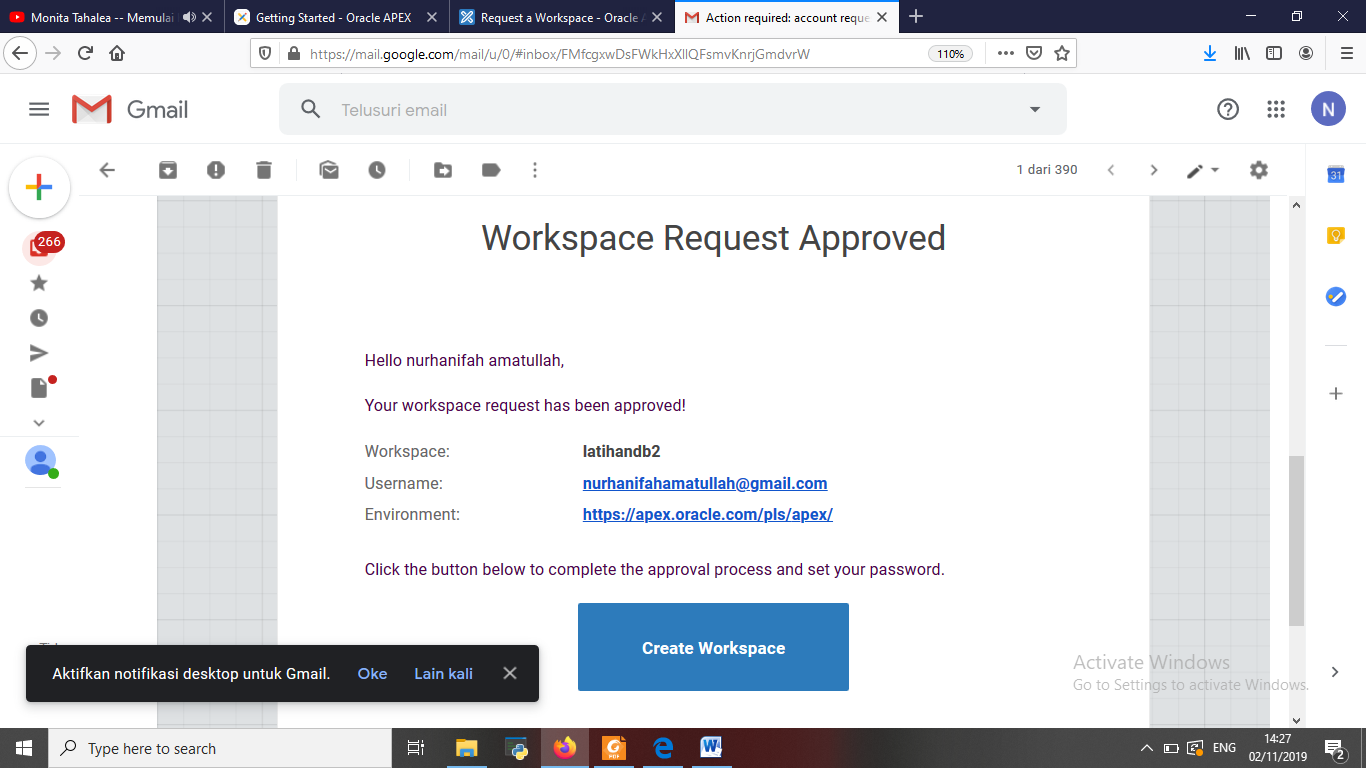
\includegraphics[scale=0.27]{gambar/6.png}
        \caption{create aplikasi}
        \label{create}
    \end{center}
    
      \item lalu pilih app builder dan pilih create
      \ref{from}
    \begin{center}
         \centering
            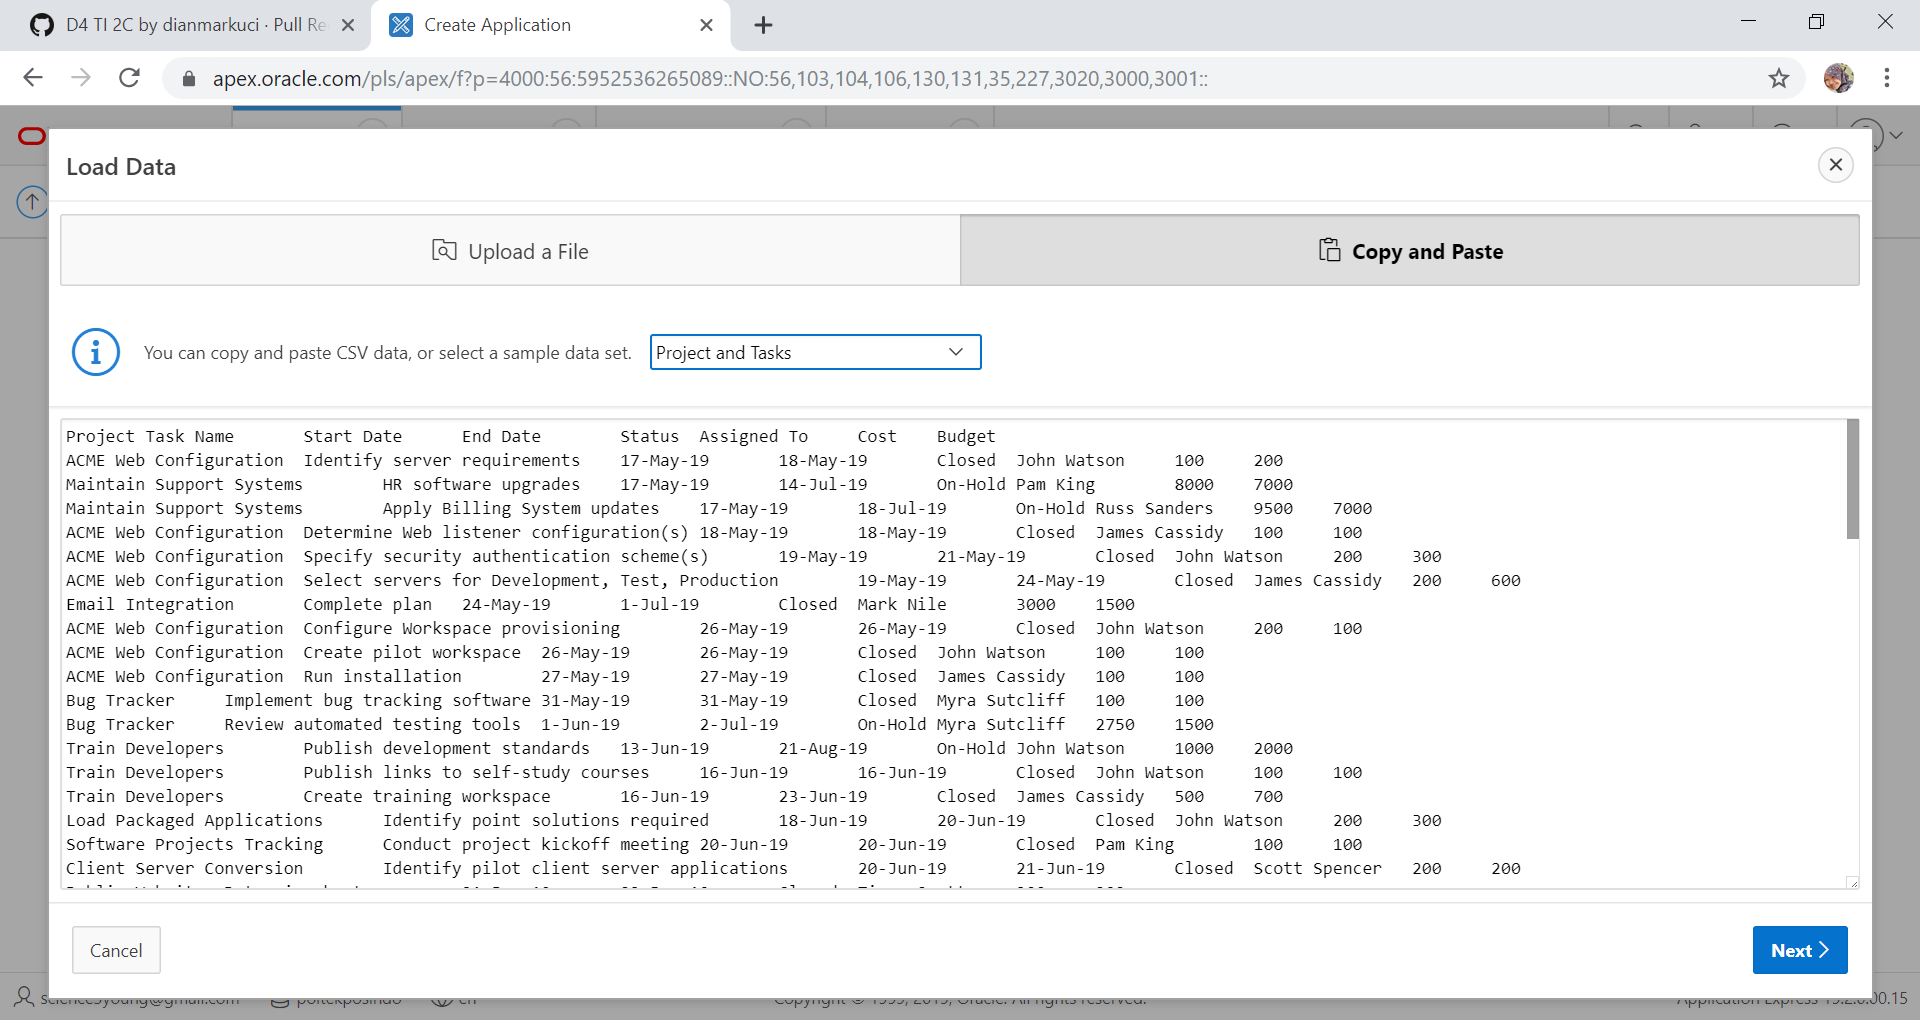
\includegraphics[scale=0.27]{gambar/7.png}
        \caption{chosse a file}
        \label{from}
    \end{center}
    
    \item 
    lalu setelah itu pilih from a file
      \ref{chosse}
    \begin{center}
         \centering
            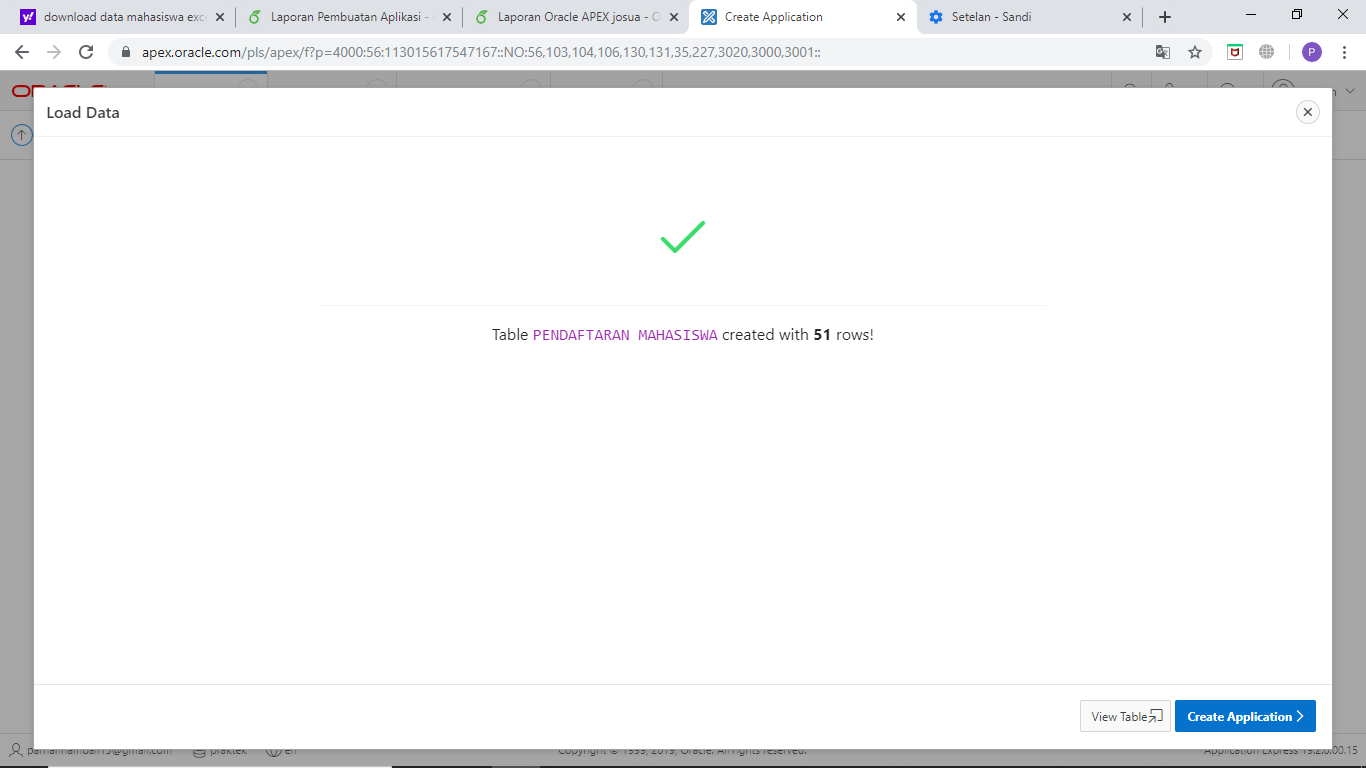
\includegraphics[scale=0.27]{gambar/8.png}
        \caption{LOAD DATA}
        \label{chosse}
    \end{center}
    
     \item lalu drag and drop
      \ref{excel}
    \begin{center}
         \centering
            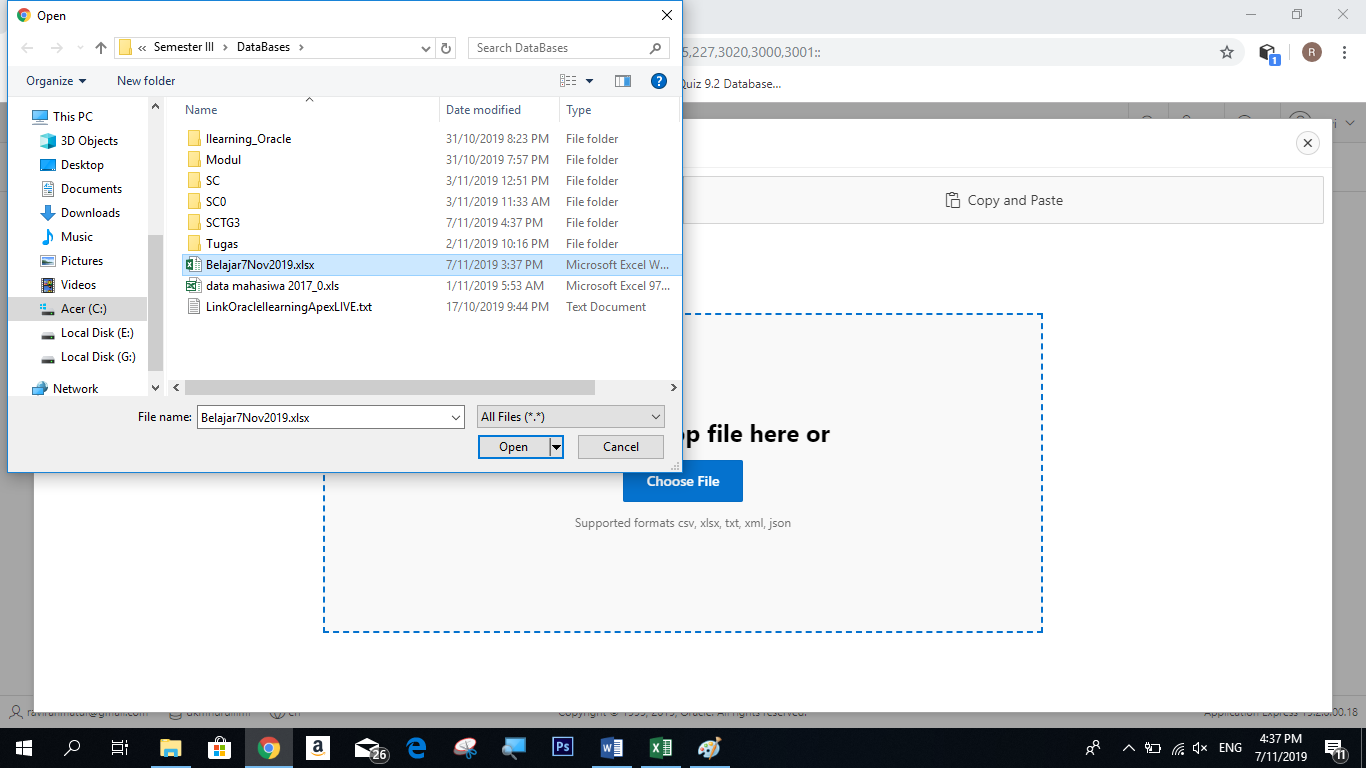
\includegraphics[scale=0.27]{gambar/9.png}
        \caption{Drag & Drop}
        \label{excel}
    \end{center}
    
     \item dan akan muncul tampilan seperti dibawah ini dan atur tabel nya sesuai nama table anda
      \ref{excel}
    \begin{center}
         \centering
            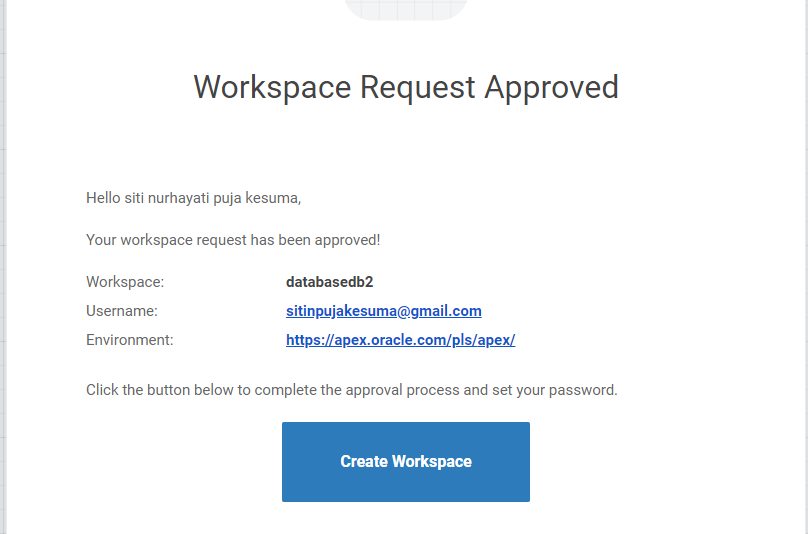
\includegraphics[scale=0.27]{gambar/10.png}
        \caption{proses create aplication}
        \label{excel}
    \end{center}
    
     \item lalu pilih configure untuk mengatur table anda
      \ref{excel}
    \begin{center}
         \centering
            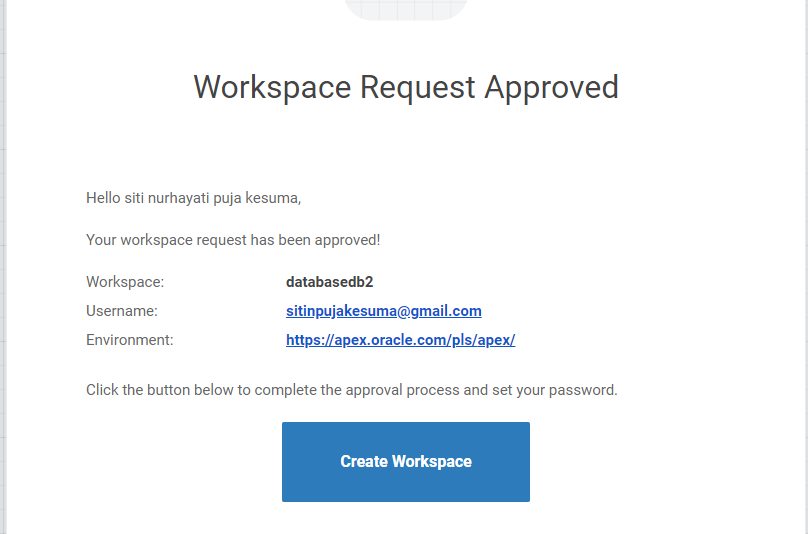
\includegraphics[scale=0.27]{gambar/10.png}
        \caption{run aplication}
        \label{excel}
    \end{center}
    
      \item dan pilih load
      \ref{excel}
    \begin{center}
         \centering
            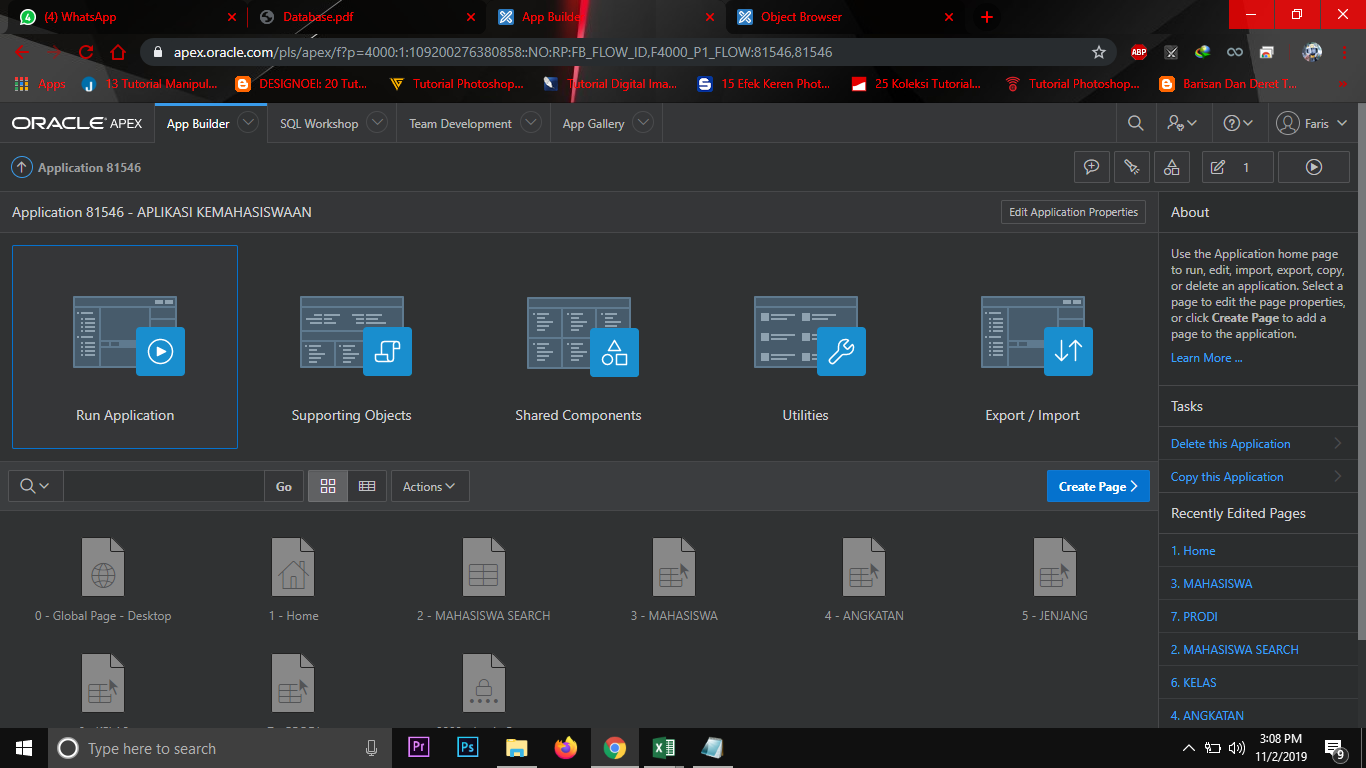
\includegraphics[scale=0.27]{gambar/11.png}
        \caption{password}
        \label{excel}
    \end{center}    
    
          \item lakukan itu pada semua table anda yang ada di excel dan masukan satu persatu dengan cara mengatur sheet nya di oracle anda


    
\end{enumerate}

\section{cara mengatur primary key dan foreign key nya}
 \begin{enumerate}
    \item sebelum membuat aplikasi kita harus terlebih dahulu menghapus id pada table anda dengan cara anda harus masuk ke sql express dan pilih object browser dan anda akan masuk ketampilan seperti dibawah ini dan anda masuk saja kedalam table anda
    

    \ref{excel}
    \begin{center}
         \centering
            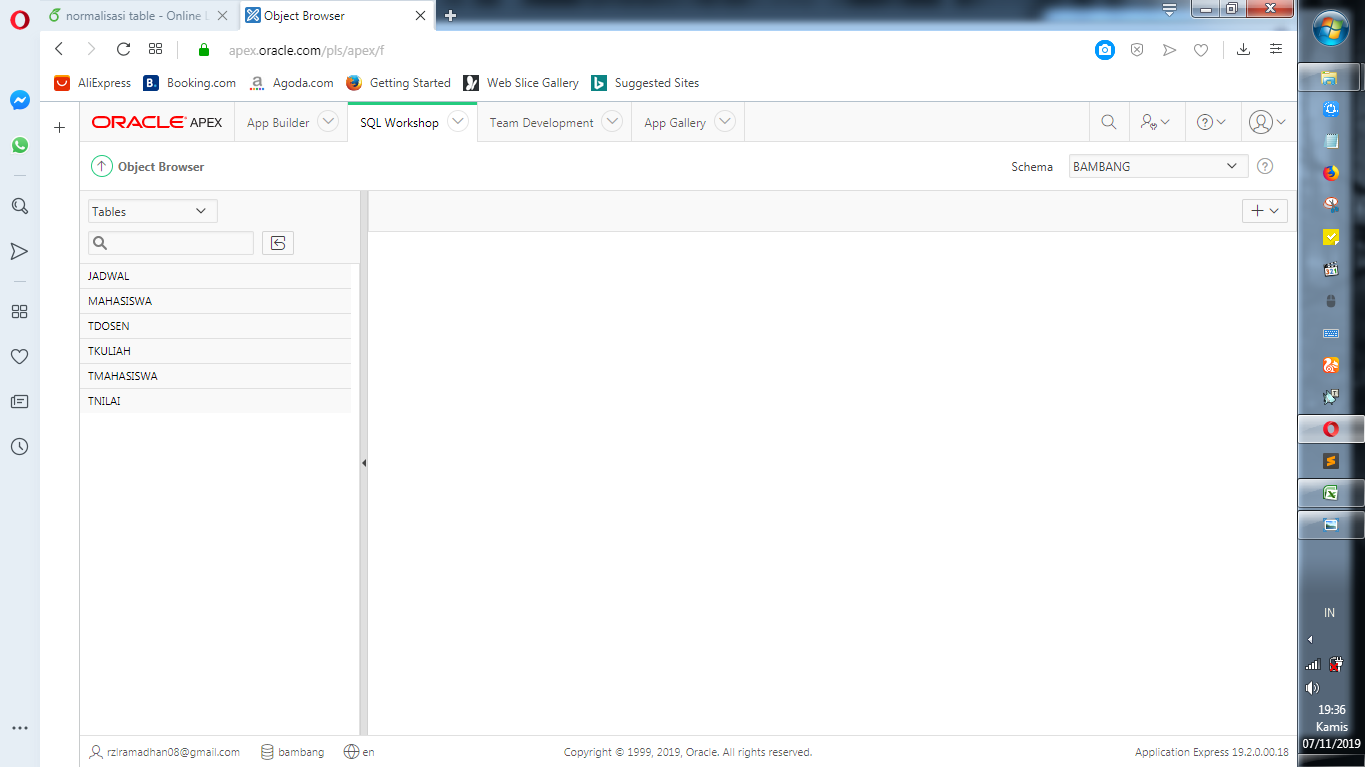
\includegraphics[scale=0.27]{gambar/12.PNG}
        \caption{Menambahkan Data}
        \label{excel}
    \end{center}

    \item lalu setelah itu anda pilih   table anda dan ubah dan pilih drop column dan lalu next saja dan di gambar yang di garis kuning apabila ada id nya next saja
    

    \ref{excel}
    \begin{center}
         \centering
            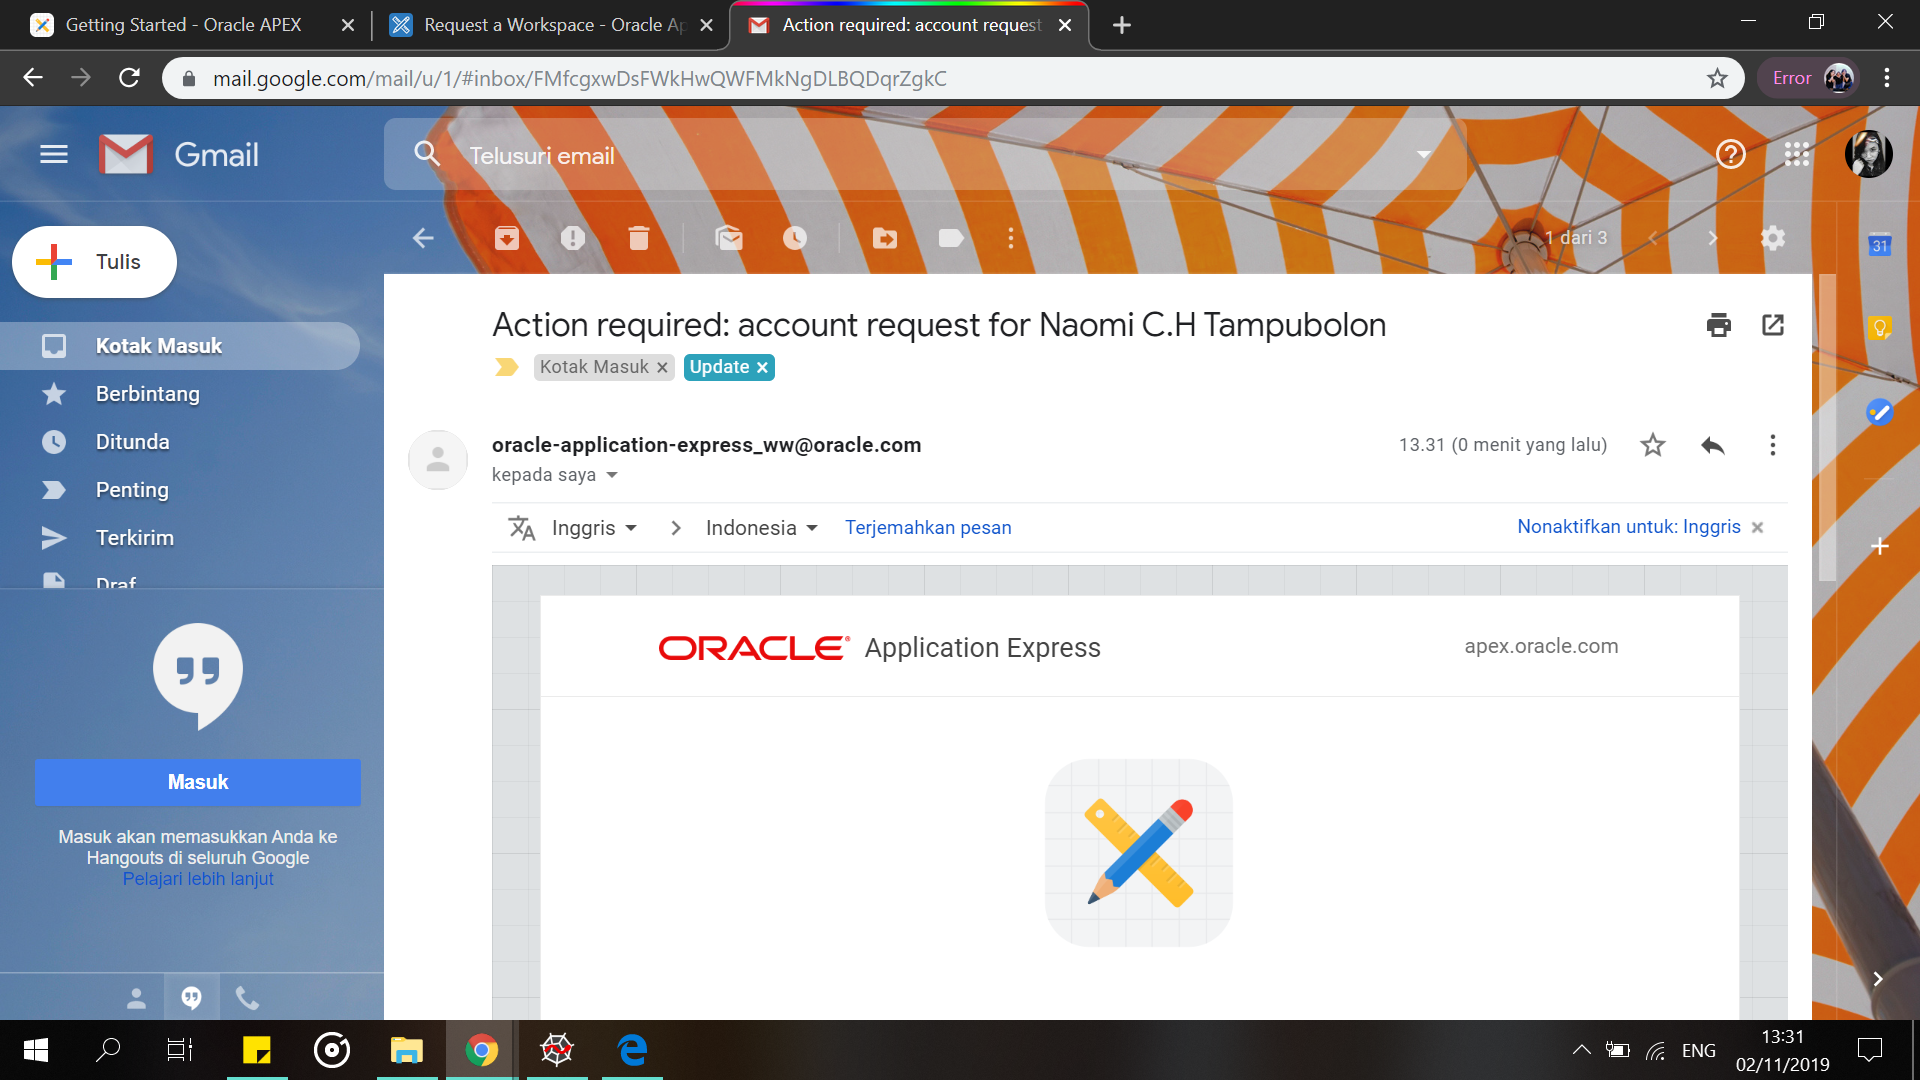
\includegraphics[scale=0.27]{gambar/13.png}
        \caption{Menambahkan Data}
        \label{excel}
    \end{center}
    
    \item lalu setelah itu lalu sql workshop dan masuk dan lalu ketikan sql commands
    
    ini berfungsi untuk membuat primary key dan apabilakoding berhasil akan ada ada alter table
    
        \ref{excel}
    \begin{center}
    
         \centering
            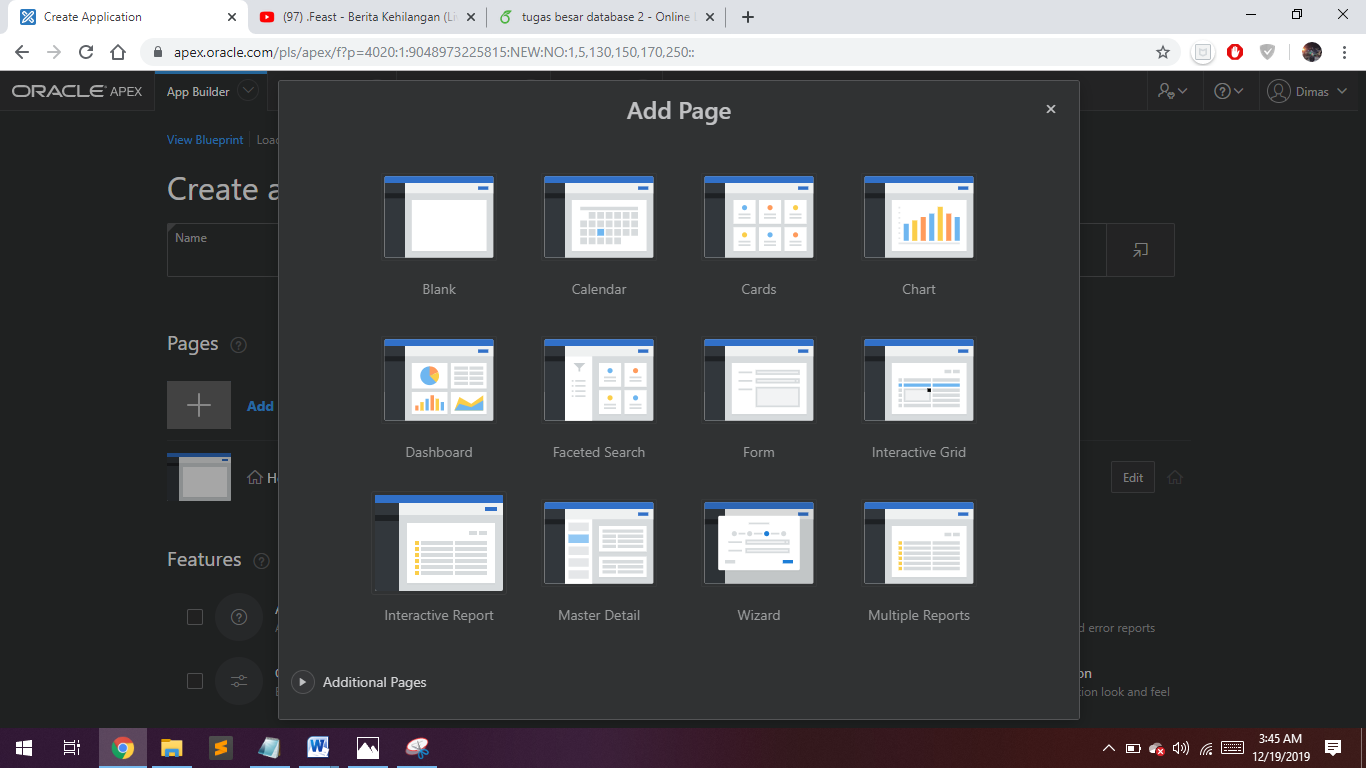
\includegraphics[scale=0.27]{gambar/14.png}
        \caption{Menambahkan Data}
        \label{excel}
    \end{center}
    
\item   setelah itu masukan cara foreign key caranya seperti dibawah ini
    \ref{excel}
    \begin{center}
         \centering
            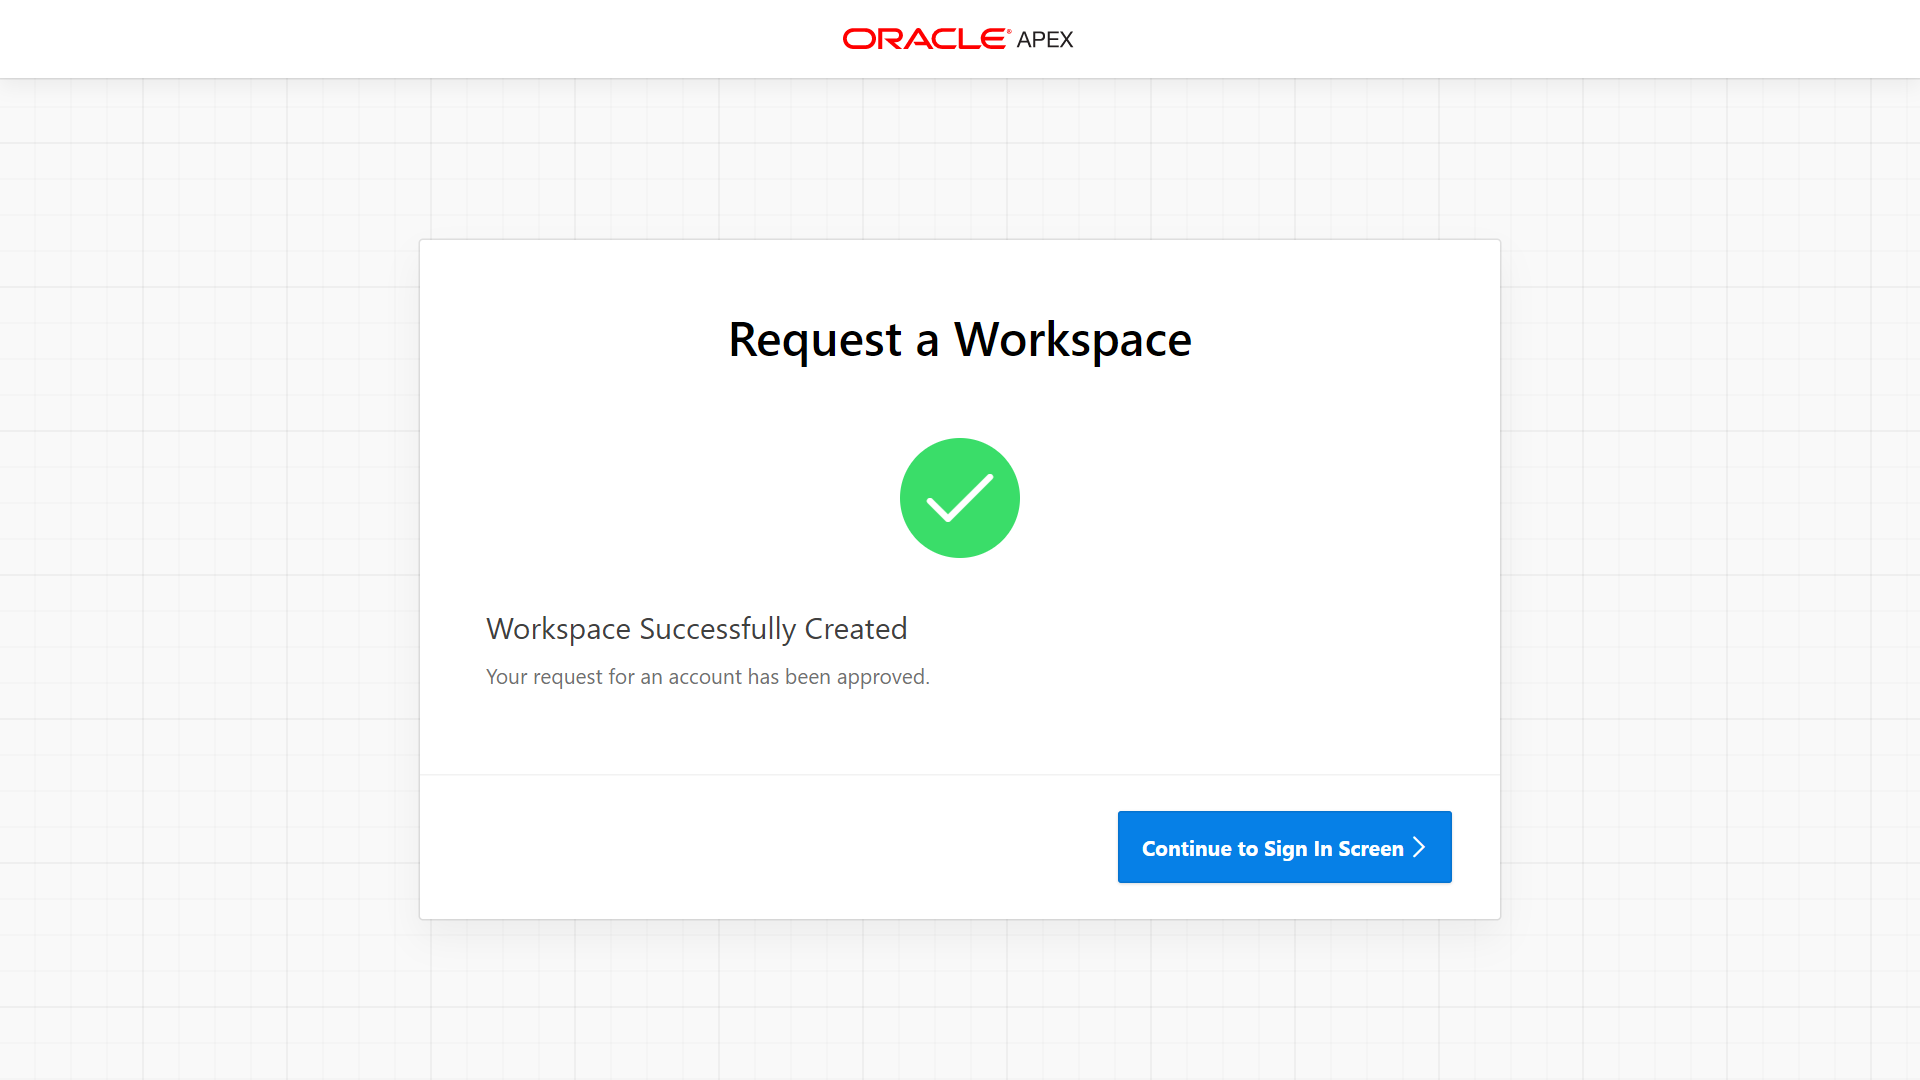
\includegraphics[scale=0.27]{gambar/15.png}
        \caption{Menambahkan Data}
        \label{excel}
    \end{center}
    
    \item setelah itu apabila anda berhasil anda cek saja di model tabl\ref{excel}
    \begin{center}
         \centering
            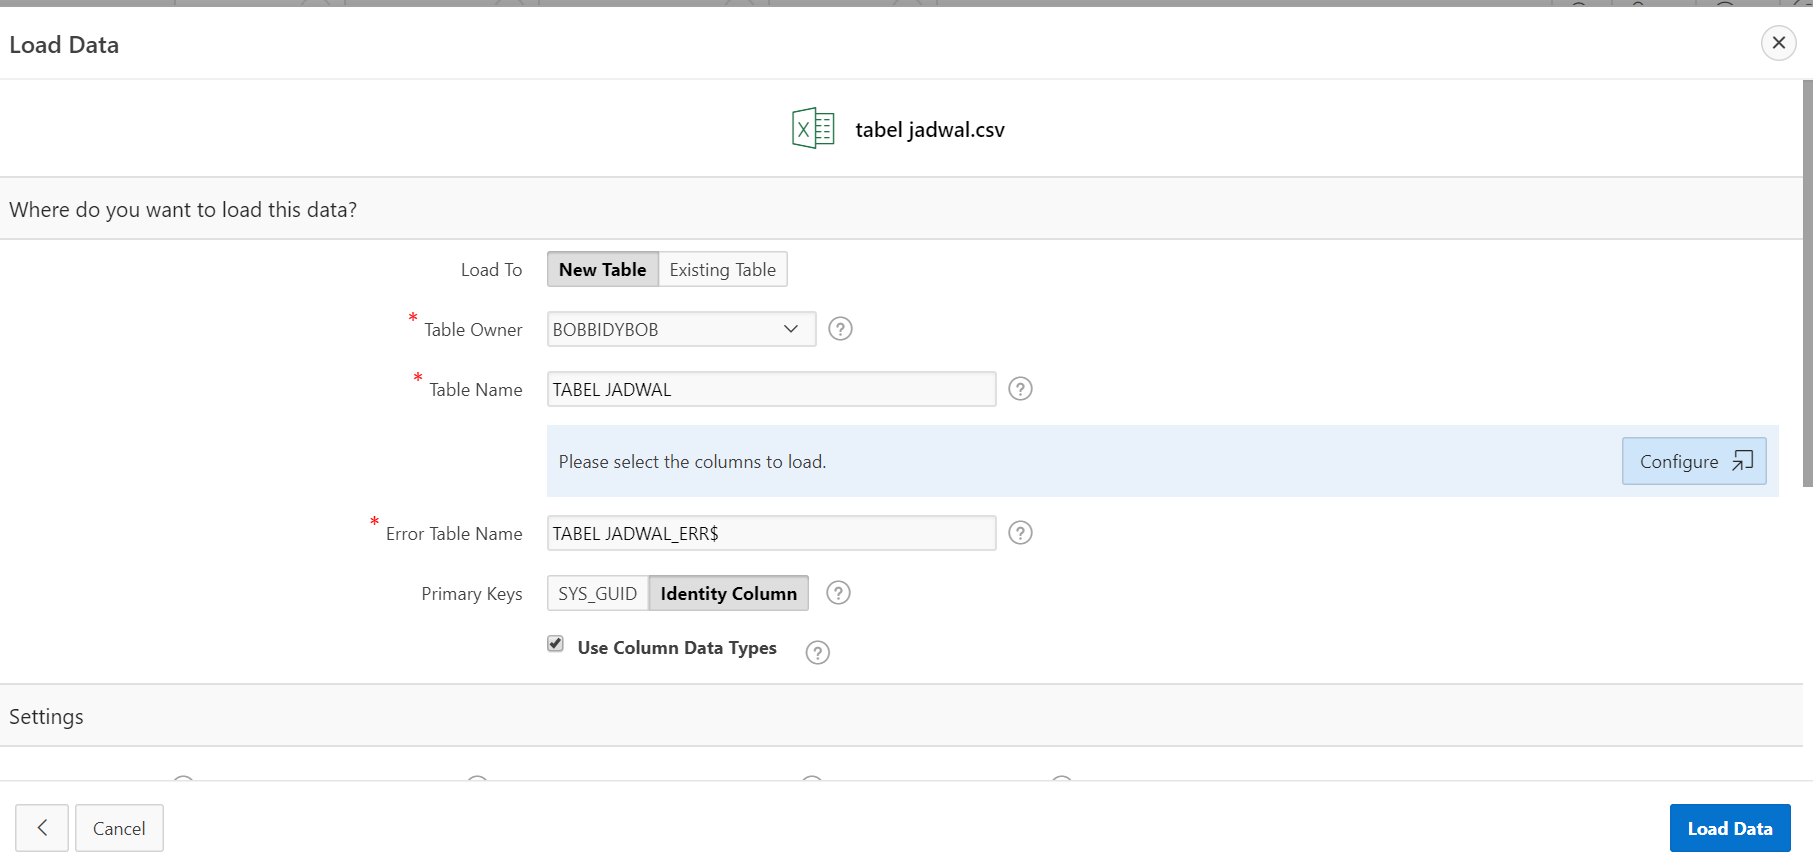
\includegraphics[scale=0.27]{gambar/16.png}
        \caption{Menambahkan Data}
        \label{excel}
    \end{center}
    
\end{enumerate}

       \section{cara membuat aplikasi nya}
 \begin{enumerate}
\item masuk app builder dan pilih create
    \begin{center}
         \centering
            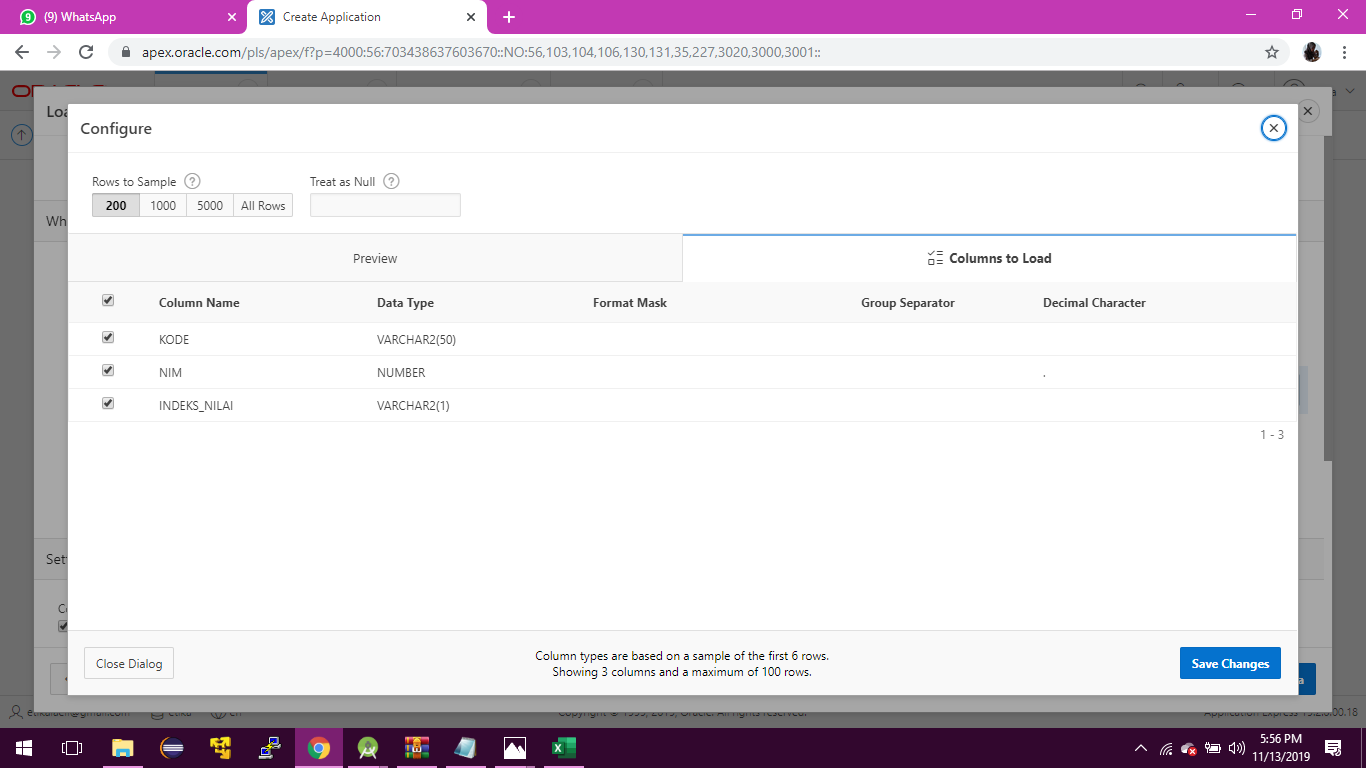
\includegraphics[scale=0.27]{gambar/17.png}
        \caption{Menambahkan Data}
        \label{excel}
    \end{center}
        
\item lalu pilih addpage dan pilih interactive report
    \begin{center}
         \centering
            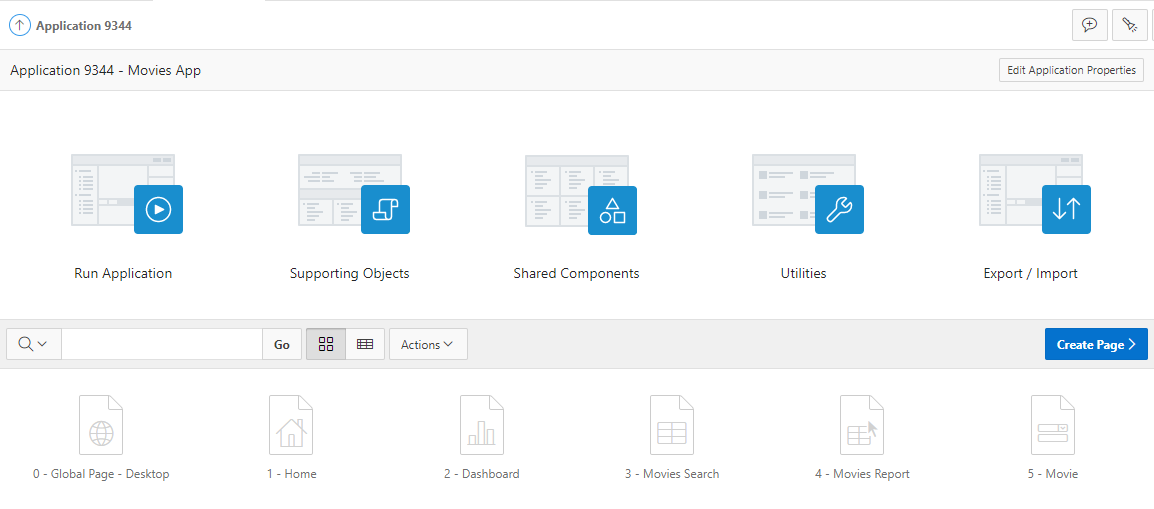
\includegraphics[scale=0.27]{gambar/18.png}
        \caption{Menambahkan Data}
        \label{excel}
    \end{center}
\item masuk app builder dan pilih create
    \begin{center}
         \centering
            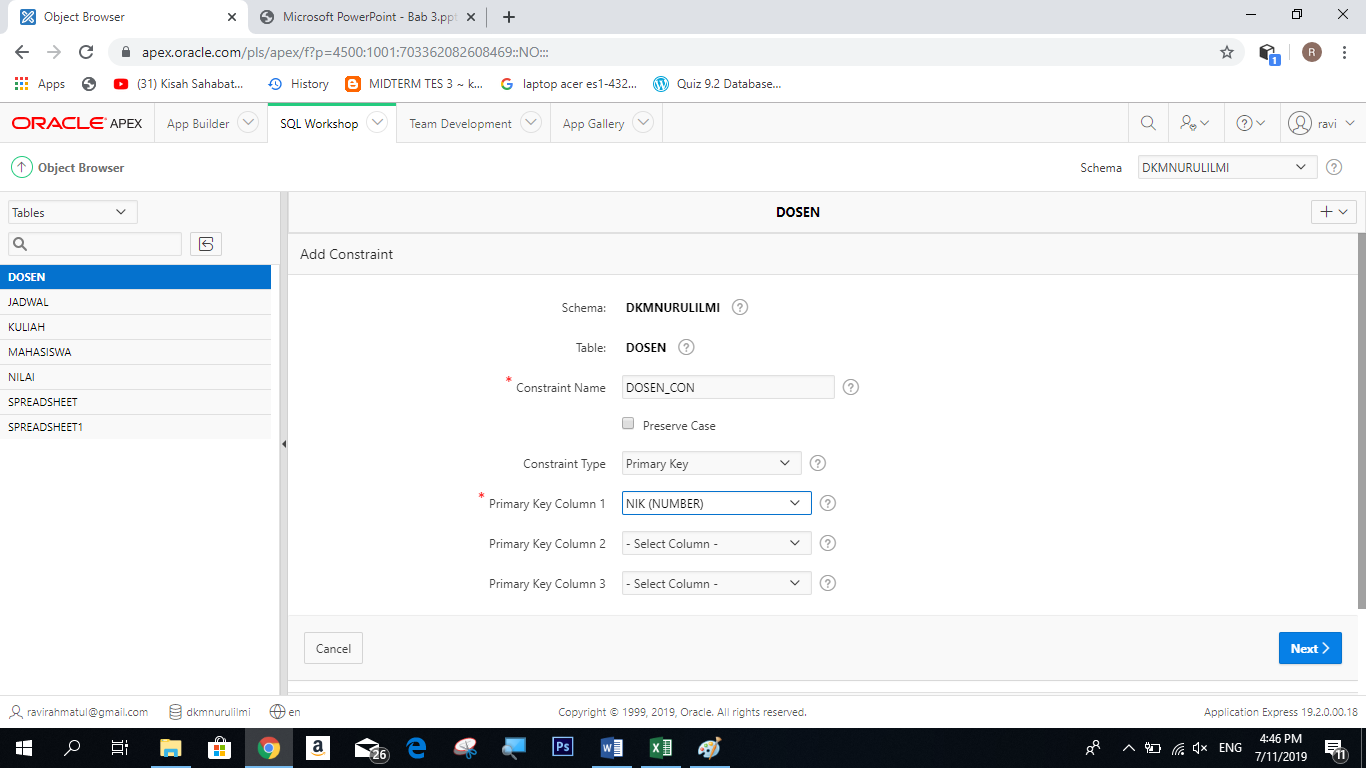
\includegraphics[scale=0.27]{gambar/19.png}
        \caption{Menambahkan Data}
        \label{excel}
    \end{center}
    
\item pilih search dialog
    \begin{center}
         \centering
            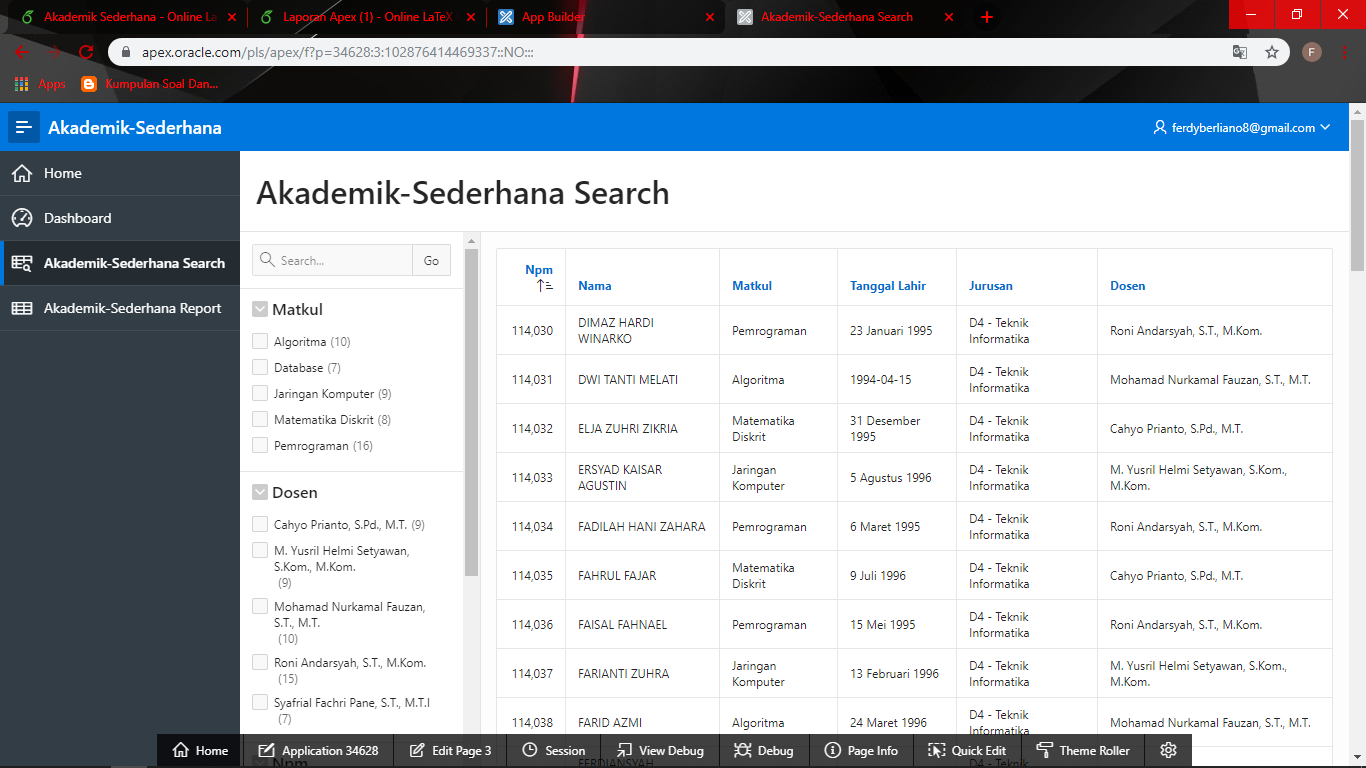
\includegraphics[scale=0.27]{gambar/20.png}
        \caption{Menambahkan Data}
        \label{excel}
    \end{center}
    
    \item pilih include form
    \begin{center}
         \centering
            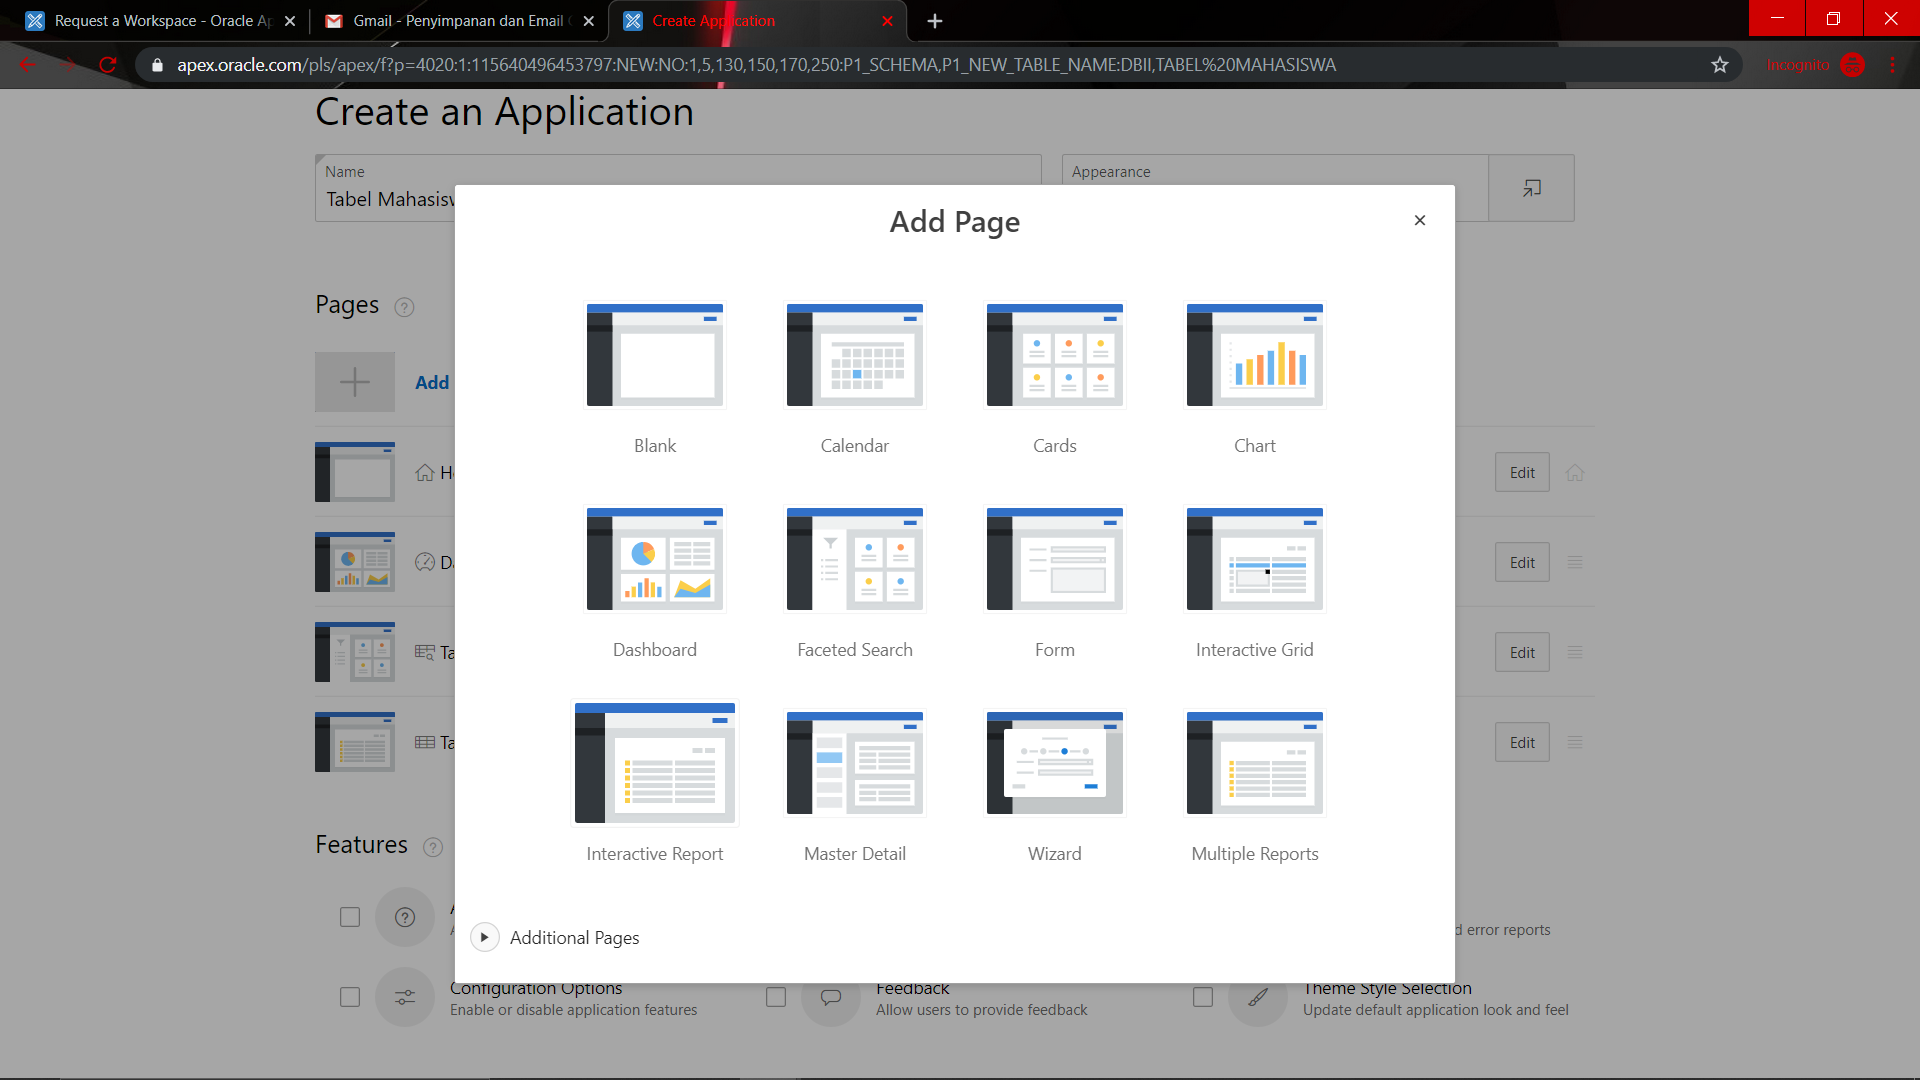
\includegraphics[scale=0.27]{gambar/21.png}
        \caption{Menambahkan Data}
        \label{excel}
    \end{center}
    
        \item masukan semua data anda seperti dibawah ini
    \begin{center}
         \centering
            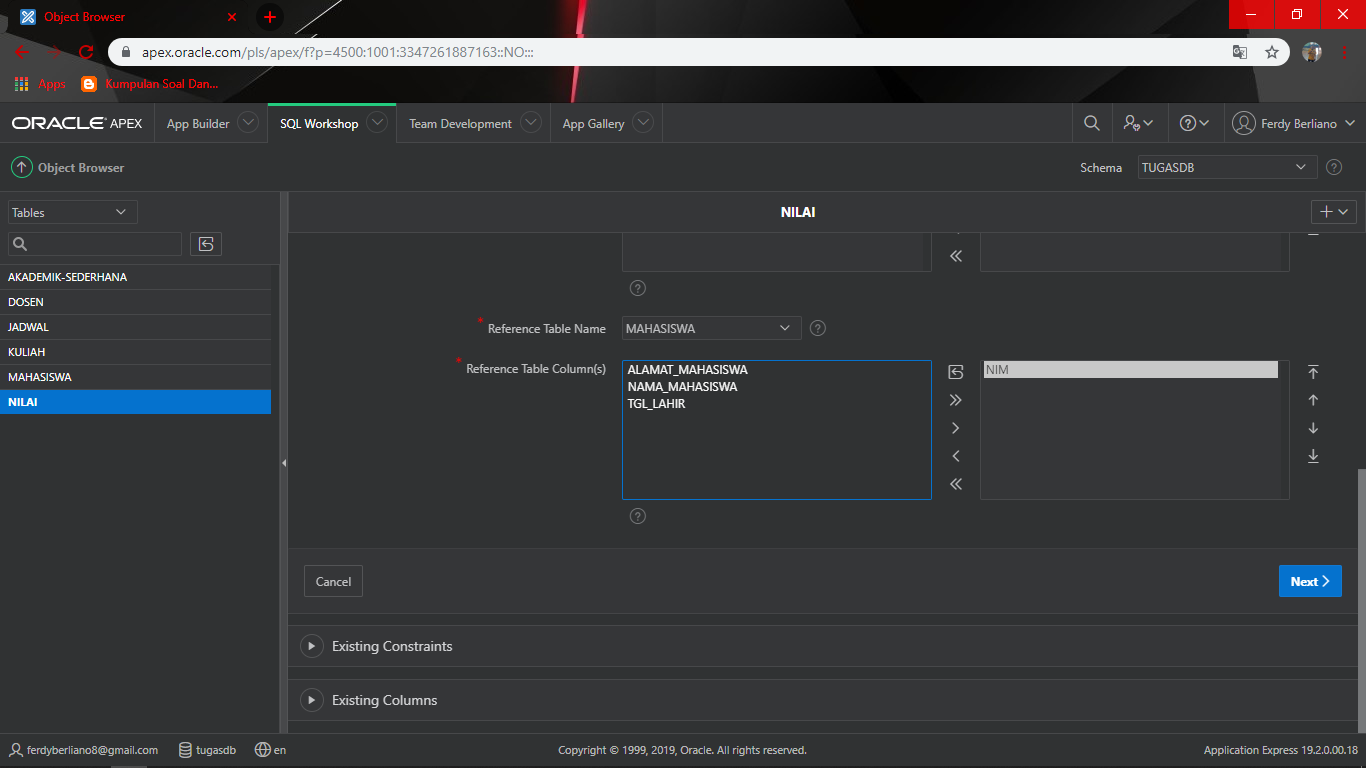
\includegraphics[scale=0.27]{gambar/22.png}
        \caption{Menambahkan Data}
        \label{excel}
    \end{center}
    
        \item pilih create aplikasi
    \begin{center}
         \centering
            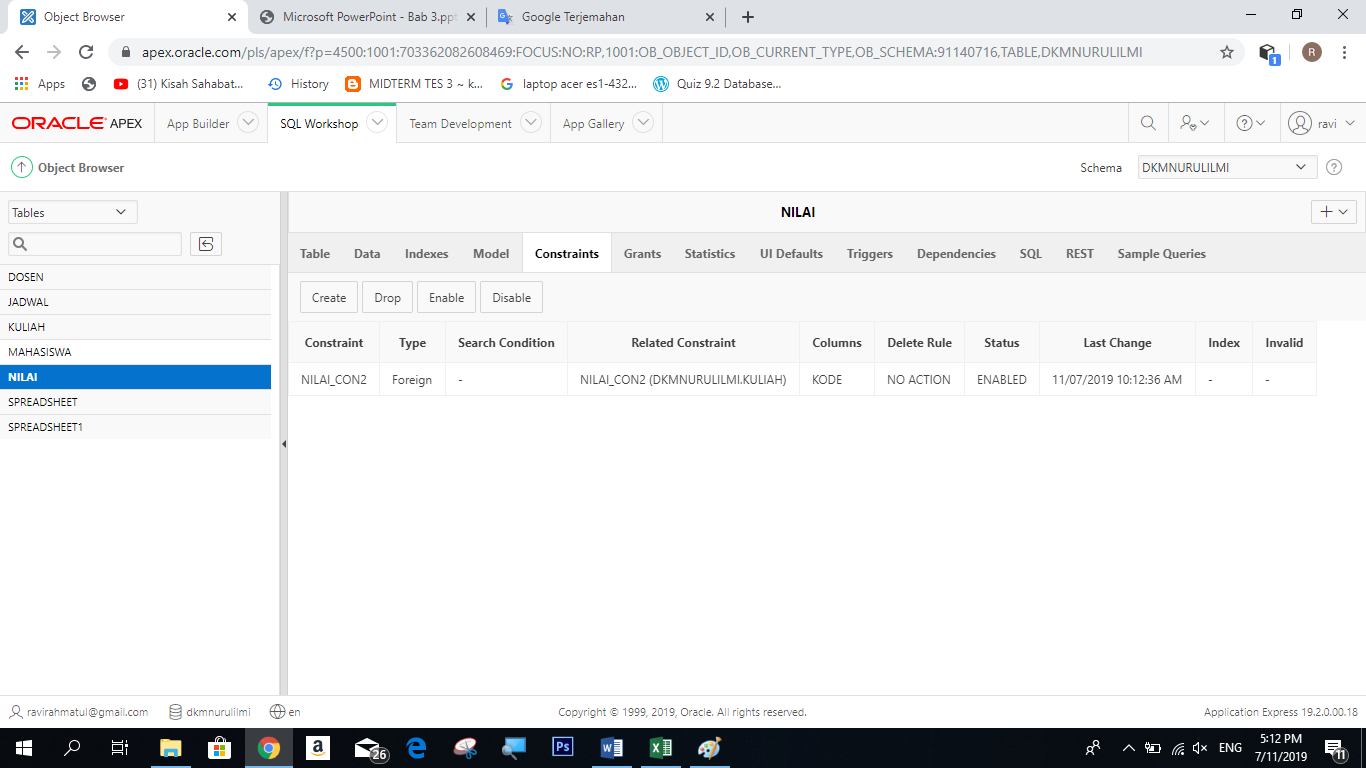
\includegraphics[scale=0.27]{gambar/23.png}
        \caption{Menambahkan Data}
        \label{excel}
    \end{center}
    
        \item pilih run aplication
    \begin{center}
         \centering
            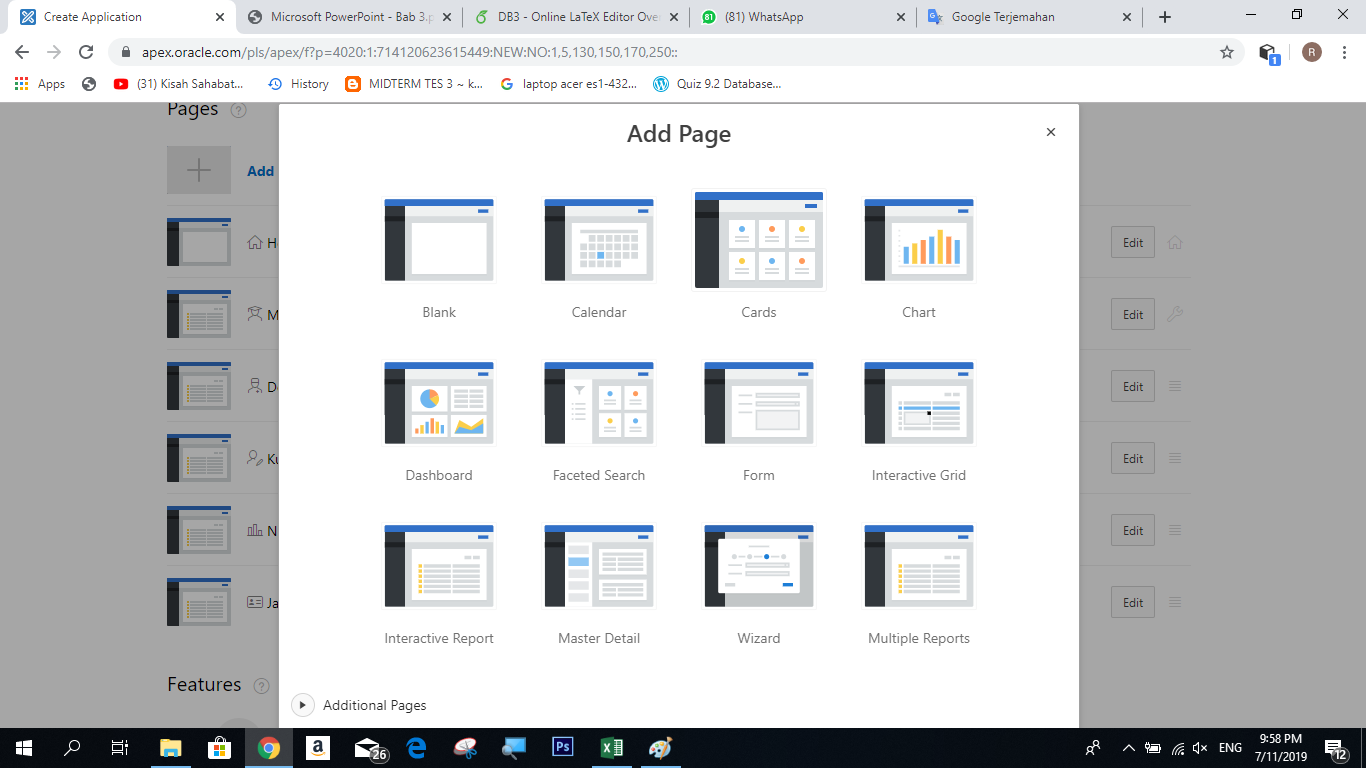
\includegraphics[scale=0.27]{gambar/24.png}
        \caption{Menambahkan Data}
        \label{excel}
    \end{center}
    
        \item login aplikasi
    \begin{center}
         \centering
            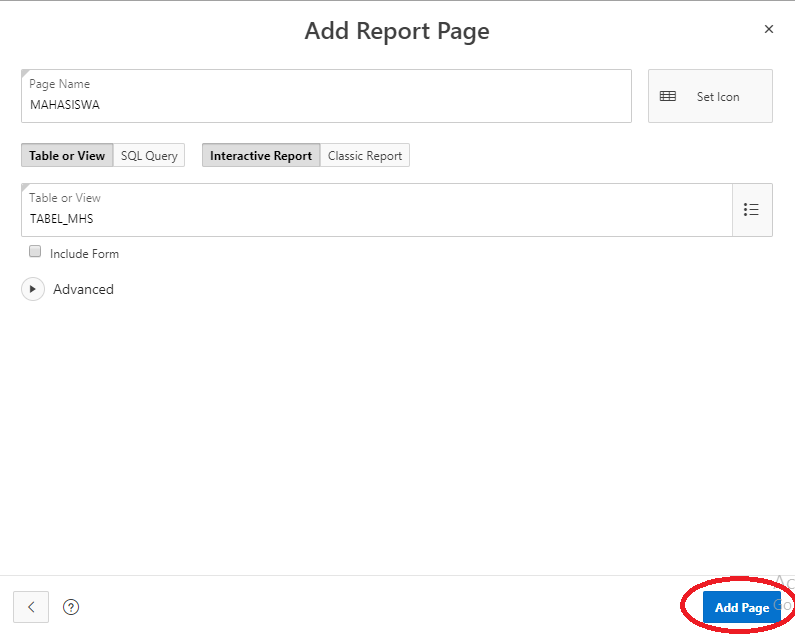
\includegraphics[scale=0.27]{gambar/25.png}
        \caption{Menambahkan Data}
        \label{excel}
    \end{center}
    
            \item tampilan aplikasi anda
    \begin{center}
         \centering
            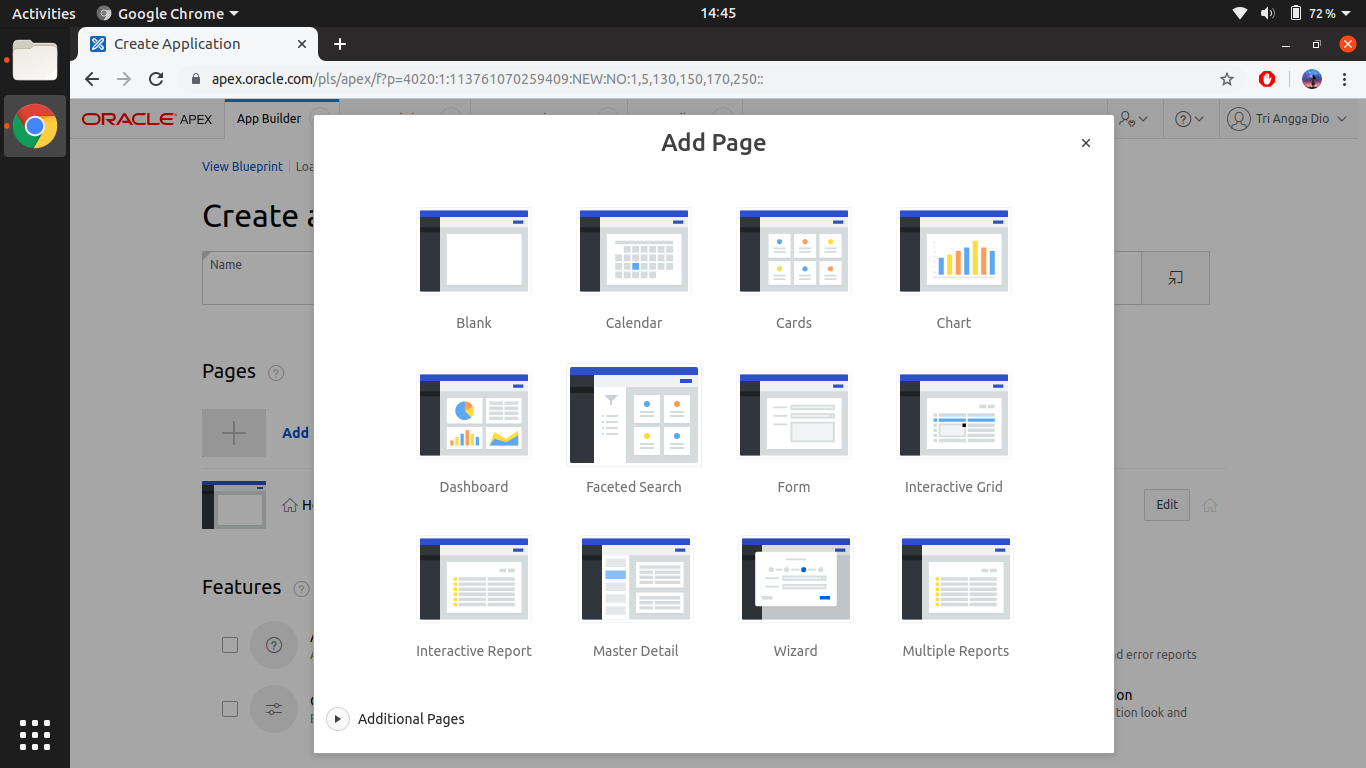
\includegraphics[scale=0.27]{gambar/26.png}
        \caption{Menambahkan Data}
        \label{excel}
    \end{center}
    
    mahasiswa
        \begin{center}
         \centering
            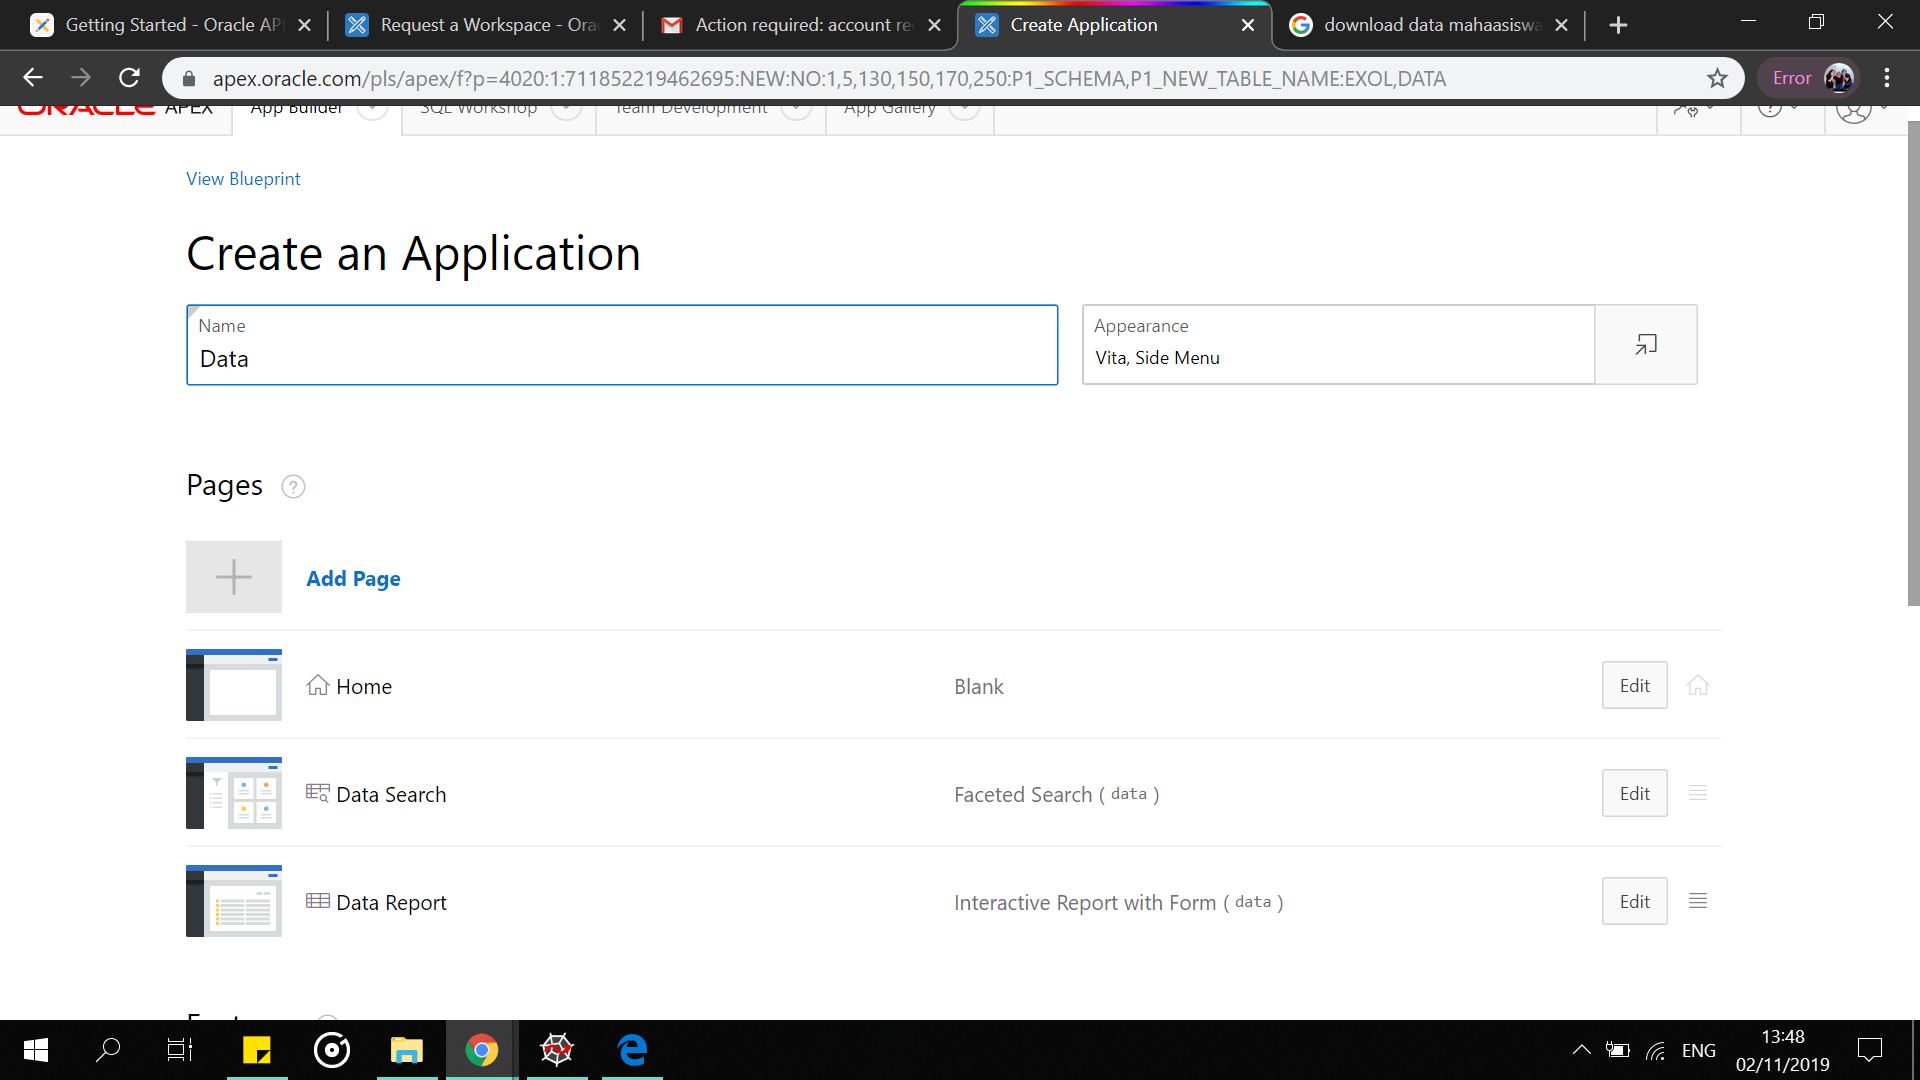
\includegraphics[scale=0.27]{gambar/27.png}
        \caption{Menambahkan Data}
        \label{excel}
    \end{center}
    
    kuliah
        \begin{center}
         \centering
            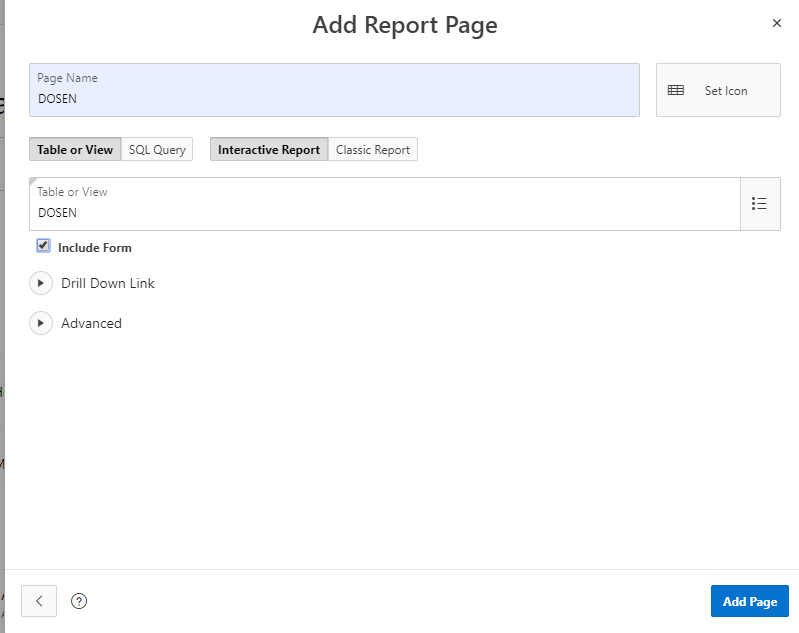
\includegraphics[scale=0.27]{gambar/28.png}
        \caption{Menambahkan Data}
        \label{excel}
    \end{center}
    
    dosen
        \begin{center}
         \centering
            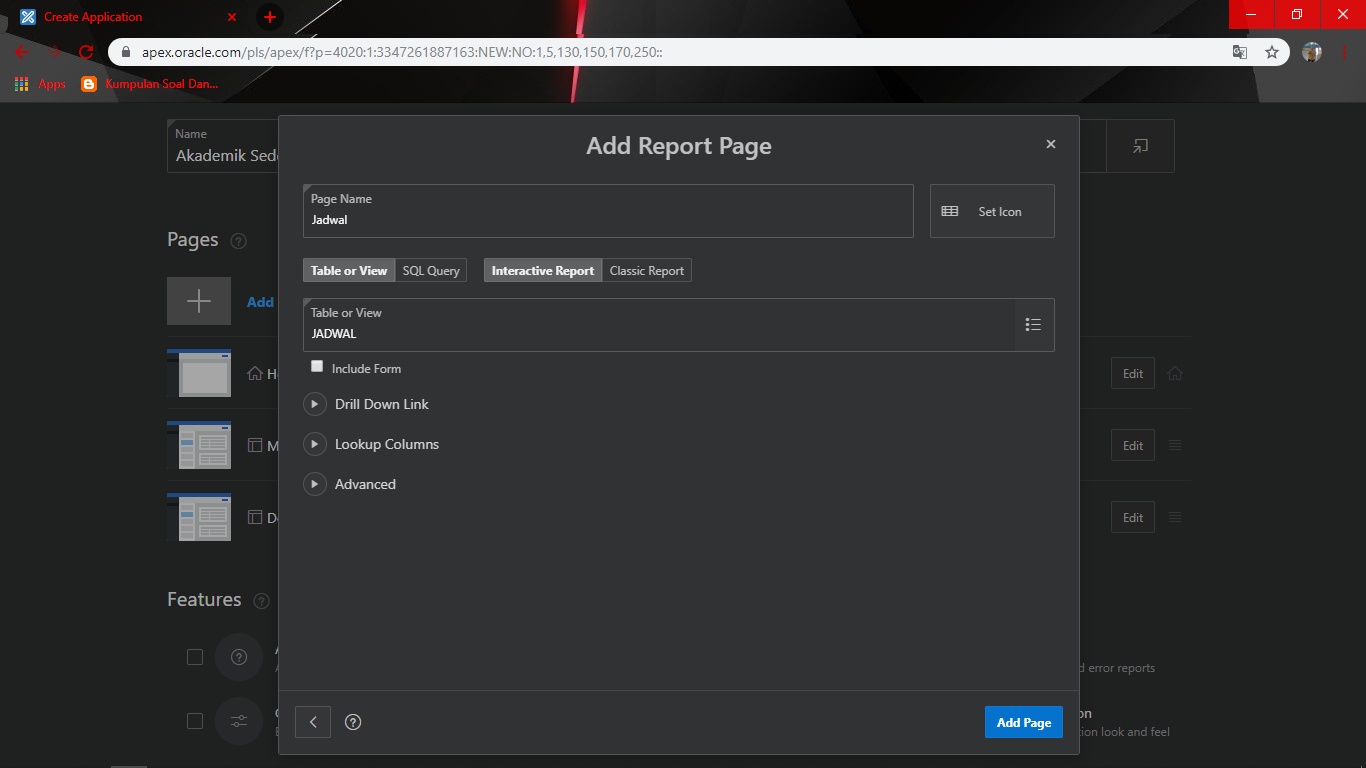
\includegraphics[scale=0.27]{gambar/29.png}
        \caption{Menambahkan Data}
        \label{excel}
    \end{center}
    
    nilai
        \begin{center}
         \centering
            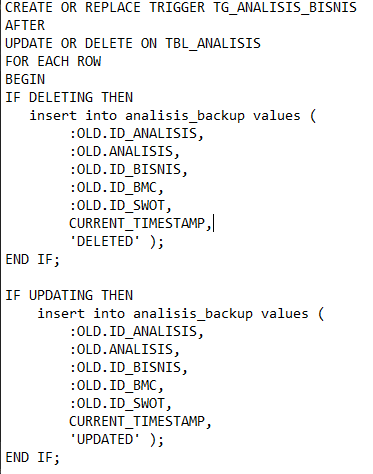
\includegraphics[scale=0.27]{gambar/30.png}
        \caption{Menambahkan Data}
        \label{excel}
    \end{center}
    
    jadwal
        \begin{center}
         \centering
            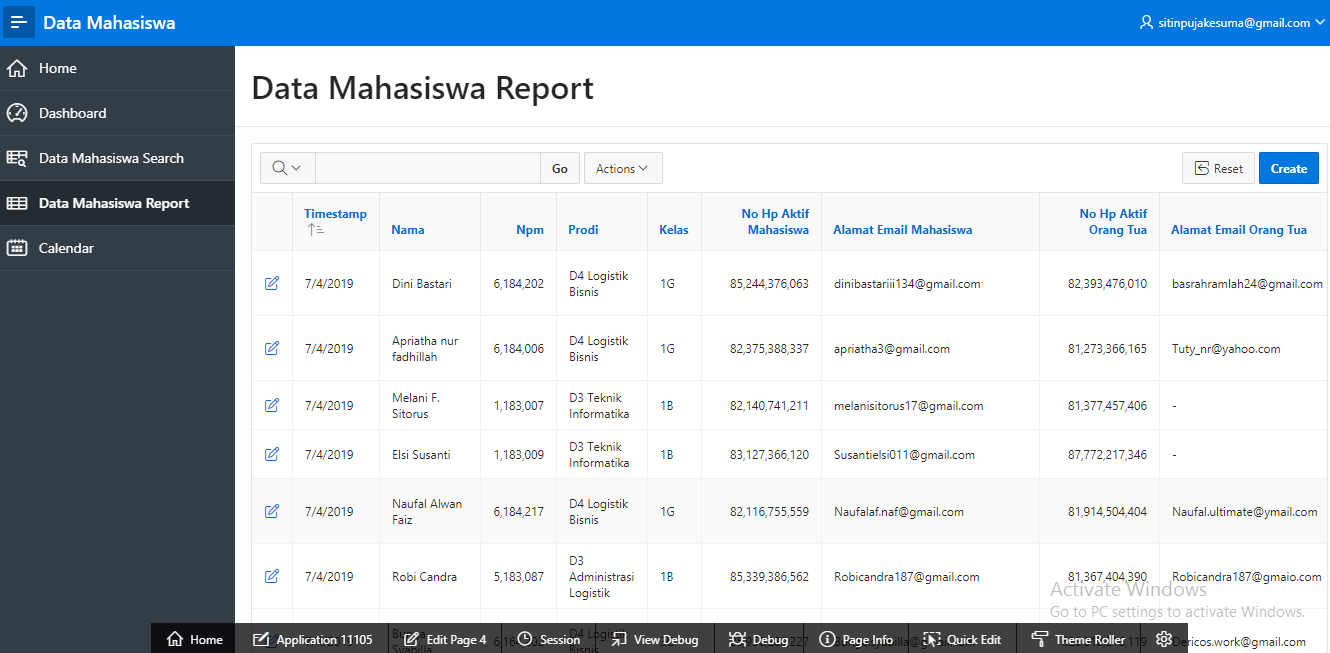
\includegraphics[scale=0.27]{gambar/31.png}
        \caption{Menambahkan Data}
        \label{excel}
    \end{center}

\end{enumerate}

\section{user dan link aplikasi}
\begin{enumerate}
\item link=https://apex.oracle.com/pls/apex/f?p=93220:1:706976331216597::NO:::
\item workspace:bambang
\item username:rzlramadhan08@gmail.com
\item password :081214488368
\end{enumerate}
\end{document}
